\documentclass[a4paper]{article}
\usepackage{import}
\usepackage[utf8]{inputenc}
\usepackage[T1]{fontenc}
\usepackage{textcomp}
\usepackage[italian]{babel}
\usepackage{amsmath, amssymb}
\usepackage{booktabs,xltabular}
\usepackage{amsfonts}
\usepackage{subcaption}
\usepackage{amsthm}
\usepackage{cancel}
\usepackage{mdframed}
\usepackage{makecell}
\usepackage{float}
\usepackage{xcolor}
\usepackage{listings}
\usepackage{gensymb}
\usepackage{graphicx}
\usepackage{bodeplot}
\usepackage{physics}
\usepackage{tikz}
\usetikzlibrary{shapes, arrows, automata, petri, decorations.markings, decorations.pathreplacing, positioning, calc, quotes}
\usepackage{circuitikz}
\usepackage[label=corner]{karnaugh-map}
\graphicspath{{./figures/}}

% Set default font to sans-serif
\renewcommand{\familydefault}{\sfdefault} 
\usepackage{eulervm}

\usepackage{forest}

\usepackage{mathtools}
\DeclarePairedDelimiter\ceil{\lceil}{\rceil}
\DeclarePairedDelimiter\floor{\lfloor}{\rfloor}

% \usepackage{ntheorem}

\usepackage{import}
\usepackage{pdfpages}
\usepackage{transparent}
\usepackage{xcolor}

\usepackage{hyperref}
\hypersetup{
    colorlinks=false,
}

% Code blocks
\definecolor{codegreen}{rgb}{0,0.6,0}
\definecolor{codegray}{rgb}{0.5,0.5,0.5}
\definecolor{codepurple}{rgb}{0.58,0,0.82}
\definecolor{backcolour}{rgb}{0.95,0.95,0.95}

\lstdefinestyle{mystyle}{
	backgroundcolor=\color{backcolour},
	commentstyle=\color{codegreen},
	keywordstyle=\color{magenta},
	numberstyle=\tiny\color{codegray},
	stringstyle=\color{codepurple},
	basicstyle=\ttfamily\footnotesize,
	breakatwhitespace=false,
	breaklines=true,
	captionpos=b,
	keepspaces=true,
	numbers=left,
	numbersep=5pt,
	showspaces=false,
	showstringspaces=false,
	showtabs=false,
	tabsize=2
}

\lstset{style=mystyle}

\usepackage{color}
\usepackage{import}
\usepackage{pdfpages}
\usepackage{transparent}
\usepackage{xcolor}

% Example frame
\theoremstyle{definition}
\newmdtheoremenv[%
	linecolor=gray,leftmargin=0,%
	rightmargin=0,
	innertopmargin=8pt,%
	innerbottommargin=8pt,
	ntheorem]{example}{Esempio}[section]

% Important definition frame
\theoremstyle{definition}
\newmdtheoremenv[%
	linecolor=gray,leftmargin=0,%
	rightmargin=0,
	backgroundcolor=gray!40,%
	innertopmargin=8pt,%
	innerbottommargin=8pt,
	ntheorem]{definition}{Definizione}[section]

% Exercise frame
\theoremstyle{definition}
\newmdtheoremenv[%
	linecolor=gray,leftmargin=0,%
	rightmargin=0,
	innertopmargin=8pt,%
	innerbottommargin=8pt,
	ntheorem]{exercise}{Esercizio}[section]

% Theorem frame
\theoremstyle{definition}
\newmdtheoremenv[%
  linecolor=gray,leftmargin=0,%
  rightmargin=0,
  innertopmargin=8pt,%
  innerbottommargin=8pt,
  ntheorem]{theorem}{Teorema}[section]

\theoremstyle{definition}
\newmdtheoremenv[%
  linecolor=white,leftmargin=0,%
  rightmargin=0,
  innertopmargin=8pt,%
  innerbottommargin=8pt,
  ntheorem]{define}{Definizione utile}[section]

% figure support
\usepackage{import}
\usepackage{xifthen}
\pdfminorversion=7
\usepackage{pdfpages}
\usepackage{transparent}
\newcommand{\incfig}[1]{%
	\def\svgwidth{\columnwidth}
	\import{./figures/}{#1.pdf_tex}
}

% FSM tikz
\tikzset{
    place/.style={
        circle,
        thick,
        draw=black,
        minimum size=6mm,
    },
        state/.style={
        circle,
        thick,
        draw=black,
        fill=white,
        minimum size=6mm,
    },
}

\pdfsuppresswarningpagegroup=1

\usepackage{pgfplots}
\pgfplotsset{compat=1.18,width=10cm}

% Save plots as pdf and reuse them without compiling every time
\usetikzlibrary{external}
\tikzexternalize[prefix=figures/tikz/, optimize=false]


% Info: 
% Libro: Fisica: Elettromagnetismo e Onde
% Esame: Scritto di 2 ore e orale facoltativo per aumentare il voto
\begin{document}
\begin{titlepage}
	\begin{center}
		\vspace*{1cm}

		\Huge
		\textbf{Probabilità e Statistica\\Esercizi}

		\vspace{0.5cm}
		\LARGE
		UniVR - Dipartimento di Informatica

		\vspace{1.5cm}

		\textbf{Fabio Irimie}

		\vfill


		\vspace{0.8cm}


		2° Semestre 2023/2024

	\end{center}
\end{titlepage}


\tableofcontents
\pagebreak

\section{Introduzione}
L'oggetto principale dello studio di questo costo è la \textbf{forza elettromagnetica}
\( \vec{F}_{em} \), più precisamente la \textbf{teoria di campo}. 

\begin{define}
  La forza è l'interazione tra due oggetti.
\end{define}

\noindent
In natura esistono solo 4 forze che governano tutto ciò che è
misurabile:
\begin{itemize}
  \item Forza di gravità (osservata quando negli oggetti interagenti c'è massa)
  \item Forza elettromagnetica (osservata quando negli oggetti interagenti c'è carica)
  \item Forza elettronucleare forte
  \item Forza elettronucleare debole
\end{itemize}
Le ultime due riguardano la materia microscopica. Le prime due invece riguardano la
materia macroscopica e sono forze \textbf{a lungo raggio}, cioè ha effetto anche
a distanza.

Lo studio della forza elettromagnetica si può fare attraverso degli strumenti
che approssimano il comportamento delle entità al livello macroscopico senza preoccuparci
della natura microscopica.

\subsection{Campo e forza}
In fisica 1 si sono studiati i concetti delle forze, cioè ciò che agisce su un corpo con
una massa, ad esempio la caduta di un grave che è attratto dalla Terra per la forza di
gravità. La visione dei campi è una visione più generale e rappresenta la proprietà
di un ambiente di interagire con un corpo, ad esempio un \textbf{campo} di gravità.

\section{Elettrostatica}
Facendo esperimenti che non sono analizzabili con i concetti della fisica 1 si arriva
a capire che c'è una nuova interazione, la \textbf{forza elettrostatica} che ha 2 forme:
\begin{itemize}
  \item Forza attrattiva
  \item Forza repulsiva
\end{itemize}
Gli oggetti sono divisi in due classi:
\begin{itemize}
  \item Carica positiva
  \item Carica negativa
\end{itemize}
Gli oggetti della stessa classe si respingono, mentre quelli di classe diversa si attraggono.
\begin{figure}[H]
  \centering
  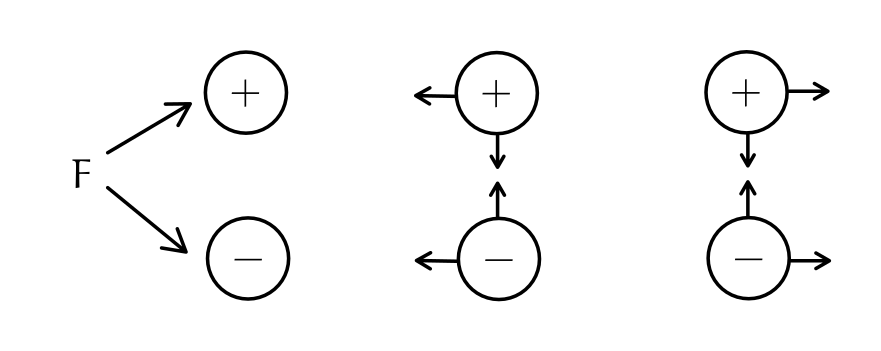
\includegraphics[width=0.8\textwidth]{tipi_carica}
  \caption{Tipi di carica}
\end{figure}
\begin{definition}[Carica elettrica]
  È chiamata \textbf{carica elettrica} \( q \) la proprietà che ha il corpo di esprimere
  la forza elettrostatica. Le proprietà di questa carica elettrica sono \textbf{indipendenti} dal
  meccanismo che l'ha generata, cioè può essere generata in modo diverso, ma ha sempre le
  stesse proprietà. Questo implica che la carica è \textbf{preesistente} in natura.
\end{definition}

\subsection{Materia}
L'atomo è formato da un nucleo centrale composto da protoni, carichi positivamente, e da
neutroni, senza carica. Intorno al nucleo si ha una regione in cui si ha la probabilità
di trovare un'altra particella, carica negativamente, chiamata elettrone.
\begin{figure}[H]
  \centering
  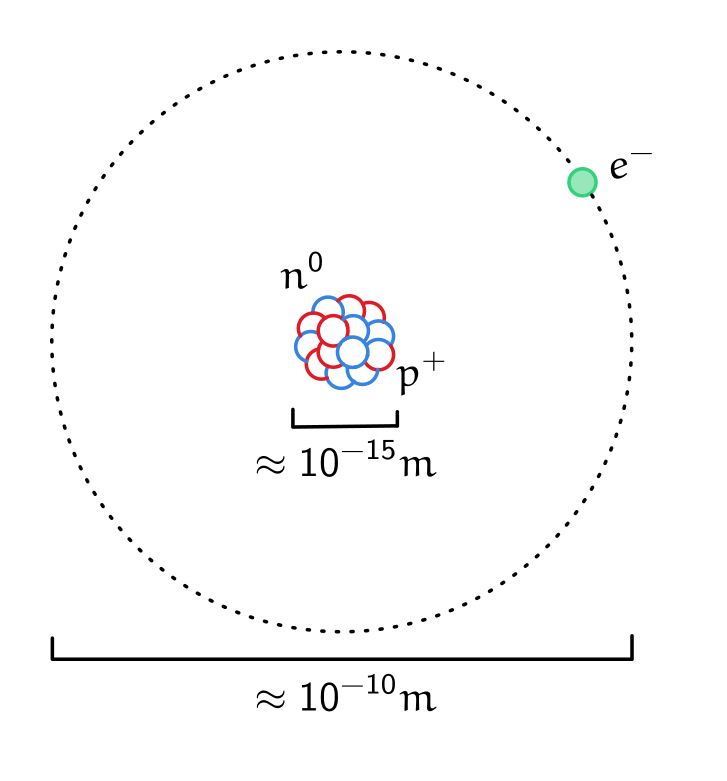
\includegraphics[width=0.6\textwidth]{atomo}
  \caption{Struttura dell'atomo}
\end{figure}
\noindent
La carica totale dell'atomo è nulla, quindi è \textbf{neutro} e
di conseguenza la carica del nucleo è uguale alla carica degli elettroni, per la precisione
il numero di protoni è uguale al numero di elettroni. \( Z \) è il numero atomico, cioè
il numero di protoni.

Elettrone e protone hanno, in modulo, la stessa carica:
\[
  |q_{e^{-}}| = q_{p^{+}}
\] 
L'elettrone è una \textbf{particella elementare}, indivisibile e la sua carica è detta
\textbf{carica elementare}, cioè la più piccola unità di carica osservabile e vale:
\[
  e^- = 1.6 \times 10^{-19}C
\] 
La \textbf{carica elettrica} in natura è quindi \textbf{quantizzata}, ovvero deve
essere un multiplo della carica dell'elettrone. Inoltre la carica non si può generare,
si può \textbf{solo trasferire}.

\begin{definition}[Legge di conservazione della carica]
  In un sistema isolato, cioè che non interagisce con altri sistemi, la carica totale 
  \( Q \) si conserva.
\end{definition}

\noindent
I componenti della materia hanno due comportamenti:
\begin{itemize}
  \item \textbf{Conduttore}: ad esempio il metallo, in cui gli elettroni sono liberi di
    muoversi
  \item \textbf{Dielettrico} (isolante): ad esempio il vetro, in cui le cariche non sono
    libere di muoversi, quindi vincolate, cioè non si riesce a strappare gli elettroni
    dall'atomo. Se si avvicina una carica positiva al dielettrico si avrà una deformazione
    delle cariche, ma non si ha una separazione di carica:
    \begin{figure}[H]
      \centering
      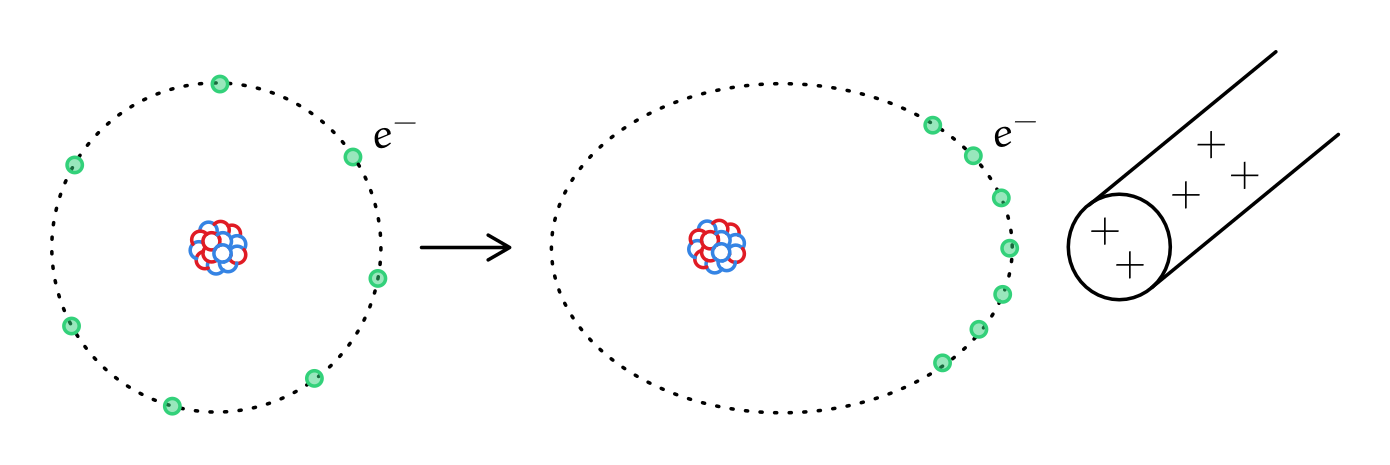
\includegraphics[width=1.0\textwidth]{dielettrico}
      \caption{Deformazione delle cariche}
    \end{figure}
    
\end{itemize}

\subsection{Elettrificazione}
L'elettrificazione è il trasferimento di carica da un corpo all'altro. Ci sono 3 
meccanismi di elettrificazione:
\begin{itemize}
  \item \textbf{Strofinio}:
    Si prende una bacchetta di vetro e un panno di lana e si strofina la bacchetta.
    La bacchetta, inizialmente, non è carica e meccanicamente con lo strofinio si strappano
    gli elettroni dagli atomi. La bacchetta diventa carica positivamente e il panno
    negativamente. Si avranno quindi le cariche \( q^+ \) della bacchetta e \( q^- \)
    del panno. Per la legge di conservazione della carica si ha:
    \[
      |q^-| = q^+
    \] 
    \begin{figure}[H]
      \centering
      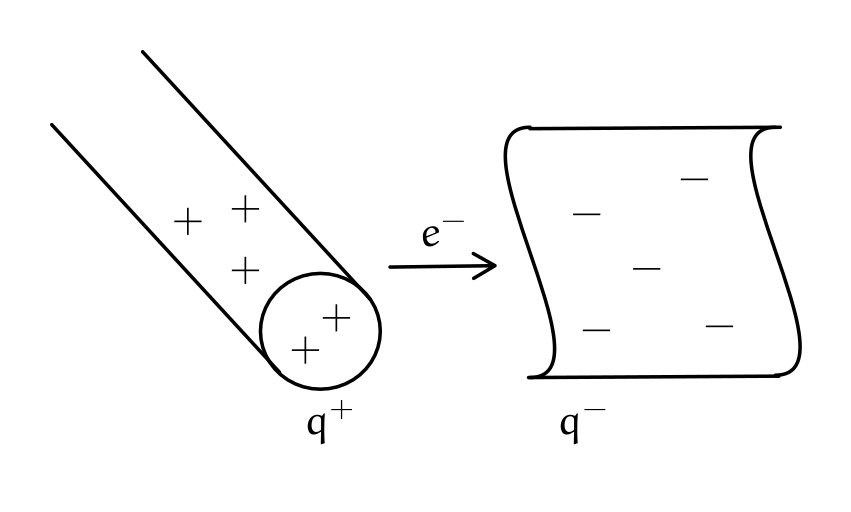
\includegraphics[width=0.7\textwidth]{strofinio}
      \caption{Strofinio}
    \end{figure}
  \item \textbf{Induzione elettrostatica}:
    Con la precedente bacchetta caricata positivamente si avvicina un oggetto metallico e
    si nota che le cariche negative \( -Q \)  del metallo si avvicinano il più possibile 
    alla bacchetta respingendo le cariche positive \( +Q \)  creando una 
    \textbf{separazione di carica per induzione}. La carica totale rimane nulla perchè 
    non sono migrati elettroni.
    \[
      |-Q| = +Q
    \] 
    \begin{figure}[H]
      \centering
      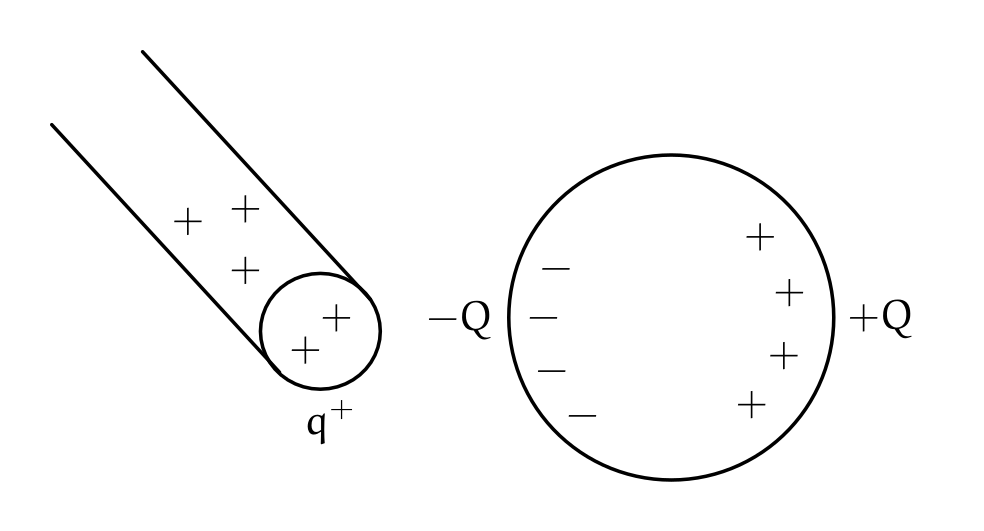
\includegraphics[width=0.7\textwidth]{induzione}
      \caption{Induzione elettrostatica}
    \end{figure}
    \noindent
    Se si allontana l'oggetto metallico si avrà una separazione meno potente.

    \vspace{1em}
    \noindent
    L'\textbf{elettroscopio} si usa per misurare la carica elettrica. È un oggetto metallico
    collegato a delle lamelle metalliche chiamate foglie:
    \begin{figure}[H]
      \centering
      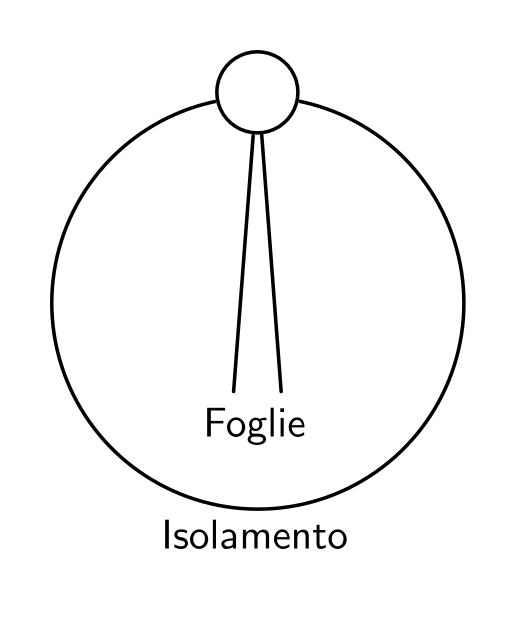
\includegraphics[width=0.4\textwidth]{elettroscopio_riposo}
      \caption{Elettroscopio}
    \end{figure}

    Si misura la carica avvicinando la bacchetta e si osserva la forza repulsiva tra le
    foglie dovuta alla repulsione tra le cariche positive della bacchetta e
    dell'elletroscopio:
    \begin{figure}[H]
      \centering
      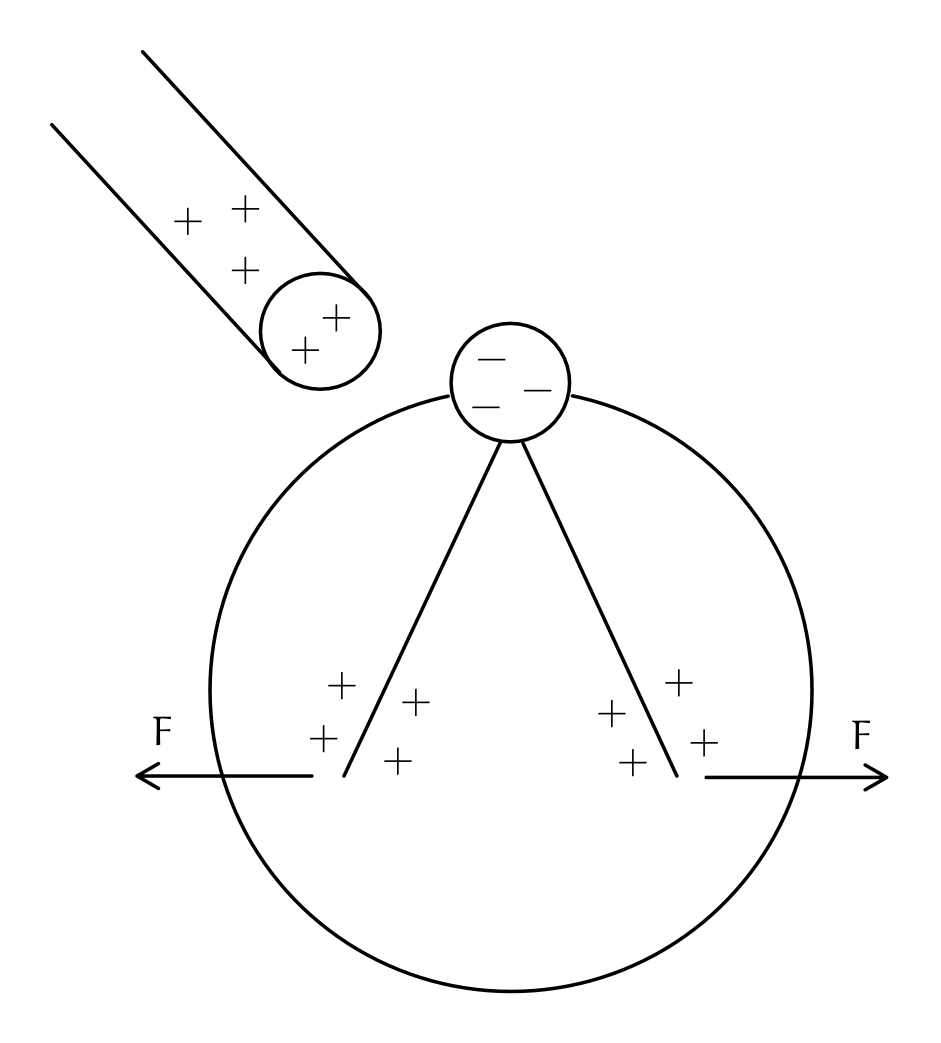
\includegraphics[width=0.5\textwidth]{elettroscopio_attivo}
      \caption{Elettroscopio durante una misurazione}
    \end{figure}
    Se si allontana la bacchetta la separazione delle foglie diminuisce.
  \item \textbf{Contatto}
    Se si prende un oggetto metallico caricato positivamente e si mette a
    contatto con un filo conduttore le cariche si sposteranno sul filo, elettrificandolo:
    \begin{figure}[H]
      \centering
      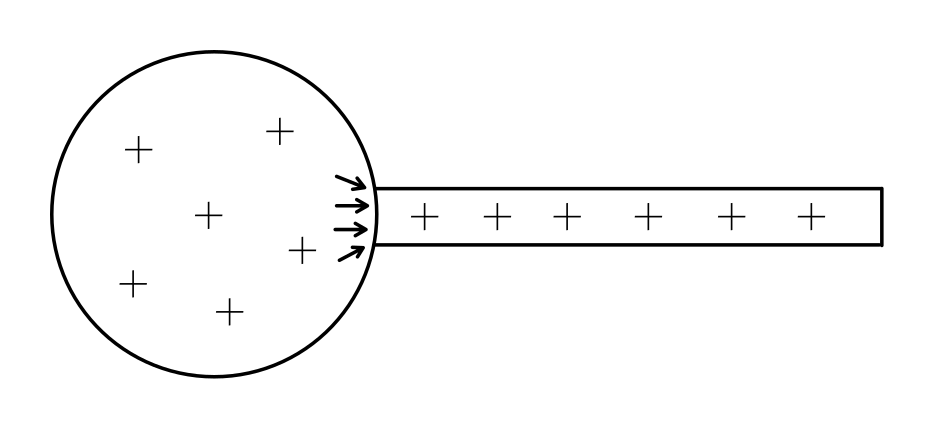
\includegraphics[width=0.7\textwidth]{contatto}
      \caption{Elettrificazione per contatto}
    \end{figure}
    Se si attacca il filo a terra l'oggetto si scarica perchè le cariche migrano verso
    la terra, cioè un conduttore immensamente più grande e quindi la carica si distribuisce
    su tutta la superficie della terra e sull'oggetto metallico rimane una carica
    \textbf{approssimativamente nulla}:
    \begin{figure}[H]
      \centering
      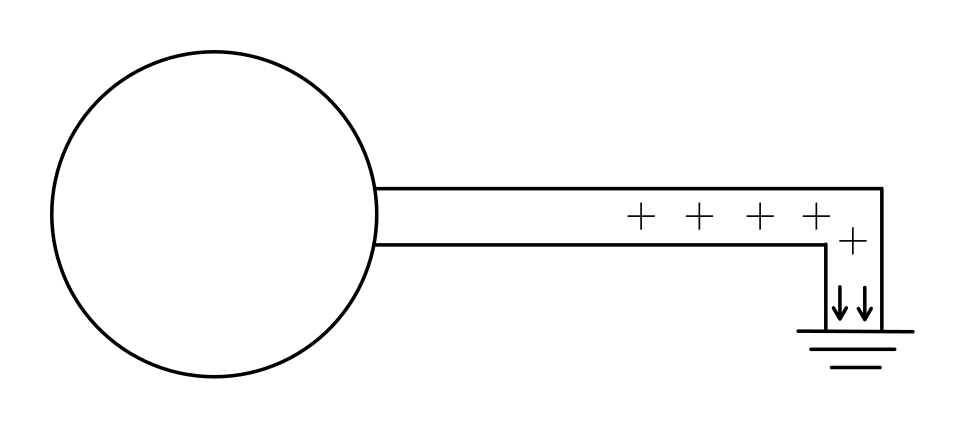
\includegraphics[width=0.7\textwidth]{contatto_terra}
      \caption{Scarica a terra}
    \end{figure}
\end{itemize}

\subsection{Elettrostatica nel vuoto}
\textbf{Fatti sperimentali}:

\vspace{1em}
\noindent
Si crea un esperimento che permette di osservare il fenomeno che si vuole modellare.
Si prende una bilancia di torsione formata da un filo torcente a cui è appesa un'asta 
con una carica \( q^+_1 \) su un'estremità. Se si avvicina una carica dello stesso
segno \( q^+_2 \) si osserva che viene applicata una forza repulsiva \( \vec{F}_{\text{el}} \)
che fa torcere il filo con un momento torcente:
\[
  \tau_{\text{filo}} = (k \theta) = \tau_{\text{el}} = \vec{d} \times \vec{F}
\]
\begin{figure}[H]
  \centering
  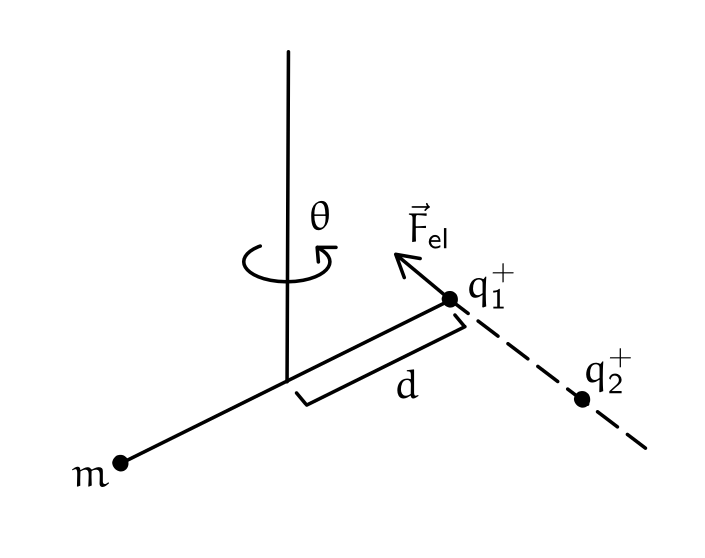
\includegraphics[width=0.7\textwidth]{bilancia_torsione}
  \caption{Bilancia di torsione}
\end{figure}
\subsubsection{Interazione di Coulomb}
Dai fatti sperimentali si nota che il modulo della forza è proporzionale al prodotto
delle cariche e inversamente proporzionale al quadrato della distanza tra le cariche:
\[
  | F_{\text{el}} | = k \frac{q_1 q_2}{r^2}
\] 
Si osserva anche che la forza elettrica \( F_{\text{el}} \) è una forza \textbf{centrale},
cioè la forza è diretta lungo la retta che congiunge le due cariche.

\( k \) è la costante di Coulomb e vale:
\[
  k = \frac{1}{4 \pi \varepsilon_0}
\]
dove \( \varepsilon_0 \) è la costante dielettrica del vuoto.
L'unità di misura della carica è il Coulomb:
\[
  [q] = C
\] 

\vspace{1em}
\noindent
Consideriamo la terna cartesiana con due cariche positive \( q^+_1 \) e \( q^+_2 \)
descritte dai raggi vettori \( \vec{r}_1 \) e \( \vec{r}_2 \). Sulla carica \( q^+_2 \) 
viene applicata una forza \( \vec{F}_{12} \) 
\begin{figure}[H]
  \centering
	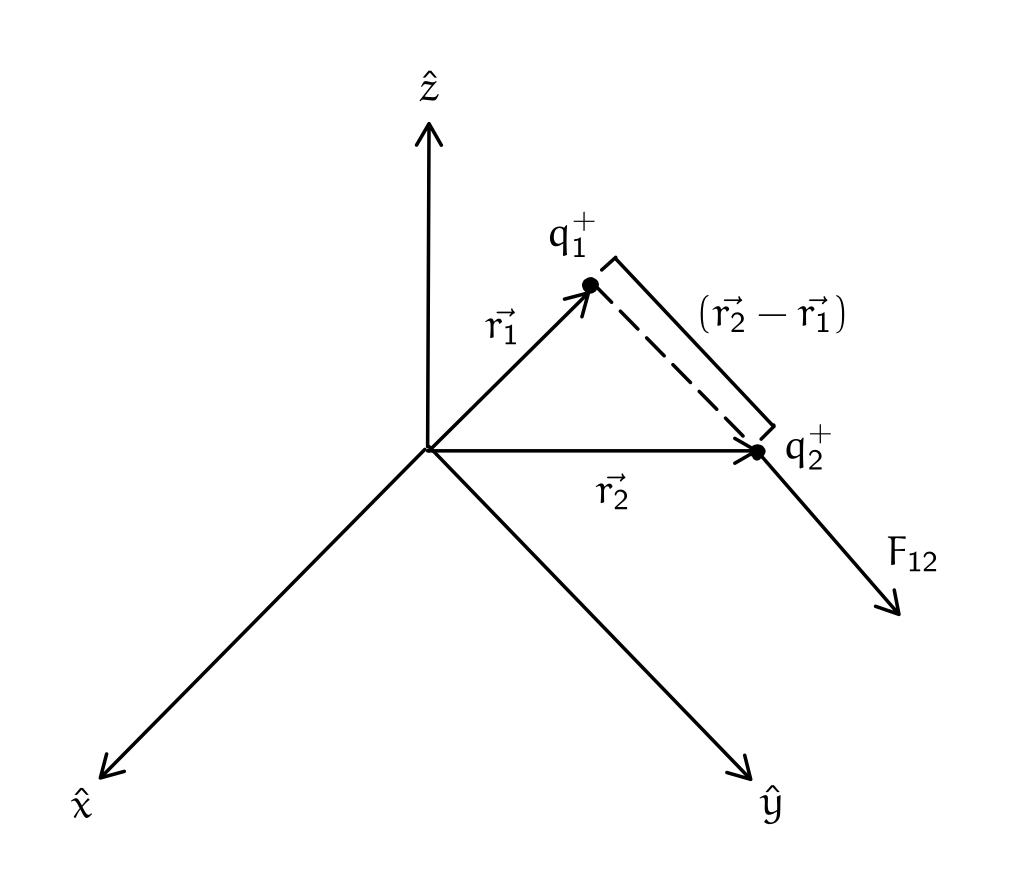
\includegraphics[width=0.7\textwidth]{forza_elettromagnetica}
  \caption{Forza elettromagnetica}
\end{figure}

\noindent
Notazione: 
\begin{itemize}
  \item 
    Chiamo il vettore che va da \( \vec{r}_1 \) a \( \vec{r}_2 \) \( \vec{r}_{12} \).

  \item 
    Il versore è indicato con \( \hat{r} \) e rappresenta il vettore unitario:
    \[
      \hat{r} = \frac{\vec{r}}{|\vec{r}|}
    \] 
\end{itemize}


\vspace{1em}
\noindent
Calcoliamo la forza \( \vec{F}_{12} \) che agisce su \( q^+_2 \) da \( q^+_1 \):
\[
  \vec{F}_{12} = \frac{1}{4 \pi \varepsilon_0} \frac{q_1 q_2}{\left( \vec{r}_{2}
    - \vec{r}_1 \right)^2} \frac{\left( \vec{r}_{2} - \vec{r}_1 \right)}{|\vec{r}_{2}
  - \vec{r}_1|} = 
  \frac{1}{4 \pi \varepsilon_0} \cdot \frac{q_1 q_2}{r_{12}^2} \cdot \hat{r}_{12} \quad [N]
\] 

\subsubsection{Sistema di più cariche}
Con più cariche si osserva che vale il principio di sovrapposizione, cioè due fenomeni
si sommano in modo lineare; e vale la terza legge di Newton, cioè l'azione-reazione
\( \left( \vec{F}_{12} = - \vec{F}_{21} \right)  \).

Consideriamo un sistema discreto con \( n \) cariche \( q_1, q_2, \ldots, q_n \) e osserviamo
la carica \( q_0 \). Ognuna di queste cariche sarà descritta dal suo raggio vettore.
\begin{figure}[H]
  \centering
  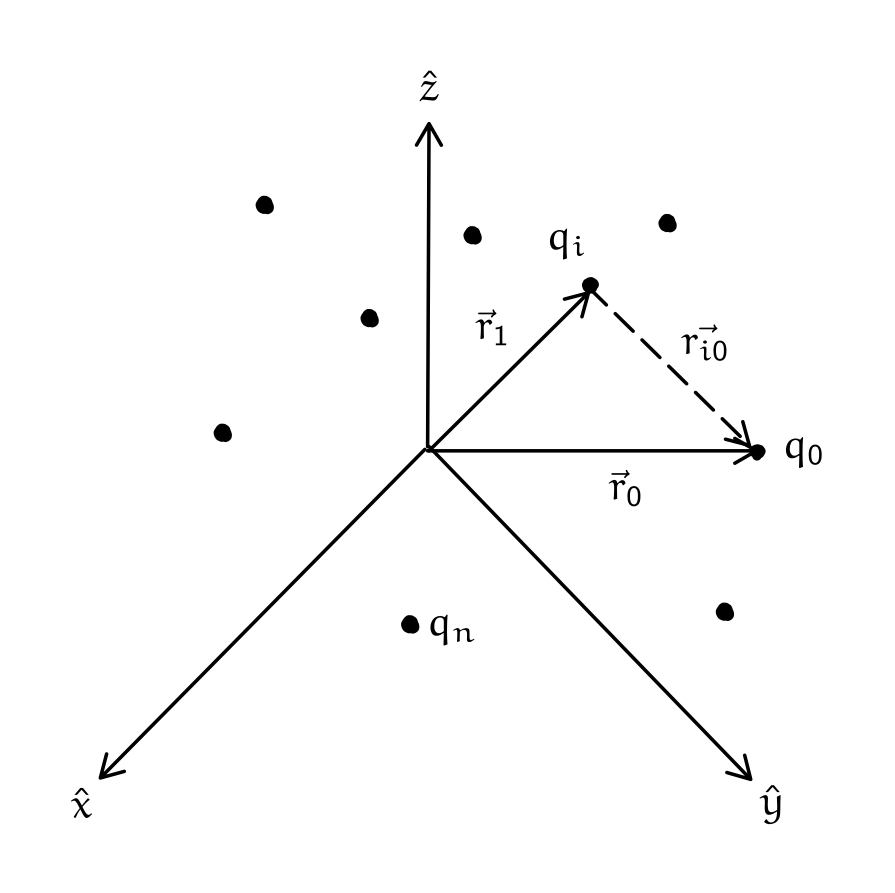
\includegraphics[width=0.7\textwidth]{forza_elettromagnetica_piu_cariche}
  \caption{Forza elettromagnetica con più cariche}
\end{figure}
\noindent
La forza che la carica \( q_i \) agisce su \( q_0 \) è:
\[
  \vec{F}_{i0} = \frac{q_i q_0}{4 \pi \varepsilon_0} \cdot \frac{\hat{r}_{i0}}{r_{i0}^2}
\] 
dove \( \vec{r}_{i0} = \vec{r}_0 - \vec{r}_i \).

Applichiamo questa formula osservando una ad una tutte le cariche come fatto per \( q_0 \)
per calcolare la forza totale applicata sulla carica \( q_0 \):
\[
  \vec{F}_{\text{tot}} = \sum_{i=1}^{n} \frac{q_i q_0}{4 \pi \varepsilon_0} \cdot 
  \frac{\hat{r}_{i0}}{r_{i0}^2} \quad \left[ N \right]
\] 
Questa forza ha direzione uguale alla somma delle forze.

\vspace{1em}
\noindent
Un'informazione si propaga con una \textbf{velocità finita}, cioè non istantaneamente. La
velocità massima di propagazione è la velocità della luce \( c \) e vale:
\[
  c = 3 \times 10^8 \, \frac{m}{s}
\]
Consideriamo lo stesso sistema di cariche, ma con la carica \( q_0 \) spostata ad una
distanza molto lontana e consideriamo le altre cariche come cariche che si muovono.
Si osserva che le cariche che si muovono cambiano il valore della forza 
\( \vec{F}_{\text{tot}} \) e dalla formula si vede che la forza cambia istantaneamente, 
ma in realtà la forza viene trasmessa dopo un tempo di propagazione (che la formula non 
tiene in considerazione).

Questa problematica si risolve con il concetto di \textbf{campo elettrostatico}.

\subsubsection{Campo elettrostatico}
Dalla formula della forza elettrostatica si può notare che la forza è proporzionale
alla carica osservata \( q_0 \):
\[
  \vec{F}_{\text{tot}} = \sum_{i=1}^{n} \frac{q_i q_0}{4 \pi \varepsilon_0} \cdot
  \frac{\hat{r}_{i0}}{r_{i0}^2} \propto q_0
\] 
Quindi la forza è proporzionale alla carica osservata e dalla distanza di questa carica:
\[
  \vec{F} = q_0 \vec{E} \left( \vec{r}_0 \right) 
\] 
Dove \( \vec{E} \) è il \textbf{campo elettrostatico} \textbf{posizionato in } \( r_0 \)
della carica osservata \( q_0 \).

\vspace{1em}
\noindent
Prendiamo in considerazione il seguente sistema in cui la particella \( Q \) è la
\textbf{sorgente di campo} e la particella \( q \) è la \textbf{carica di prova}:
\begin{figure}[H]
  \centering
  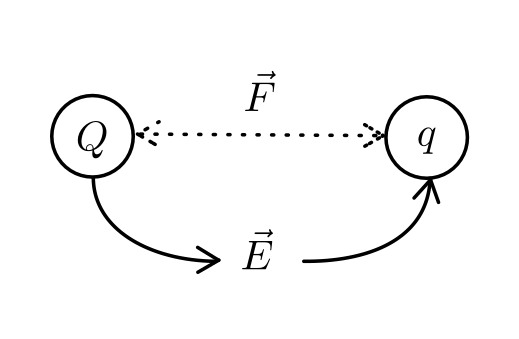
\includegraphics[width=0.6\textwidth]{campo_elettrostatico}
  \caption{Campo elettrostatico}
\end{figure}
\[
    \vec{F} = q \vec{E} \left( \vec{r} \right)
\] 
\[
  \vec{E} \left( r \right) = \frac{\vec{F}}{q}
\] 
Questa è la \textbf{definizione operativa} di campo, cioè serve una carica di prova per
misurare il campo.

\begin{definition}
  Il campo di una singola carica puntiforme \( Q \), posizionata per comodità nell'origine,
  considerata una particella di test \( q \) ad una distanza \( \vec{r} \) è definito come:
  \[
    \vec{E}( \vec{r} ) = \frac{Q}{4 \pi \varepsilon_0} \cdot \frac{\hat{r}}{r^2}
    \quad \left[ \frac{N}{C} \right]
  \] 
  \begin{figure}[H]
    \centering
    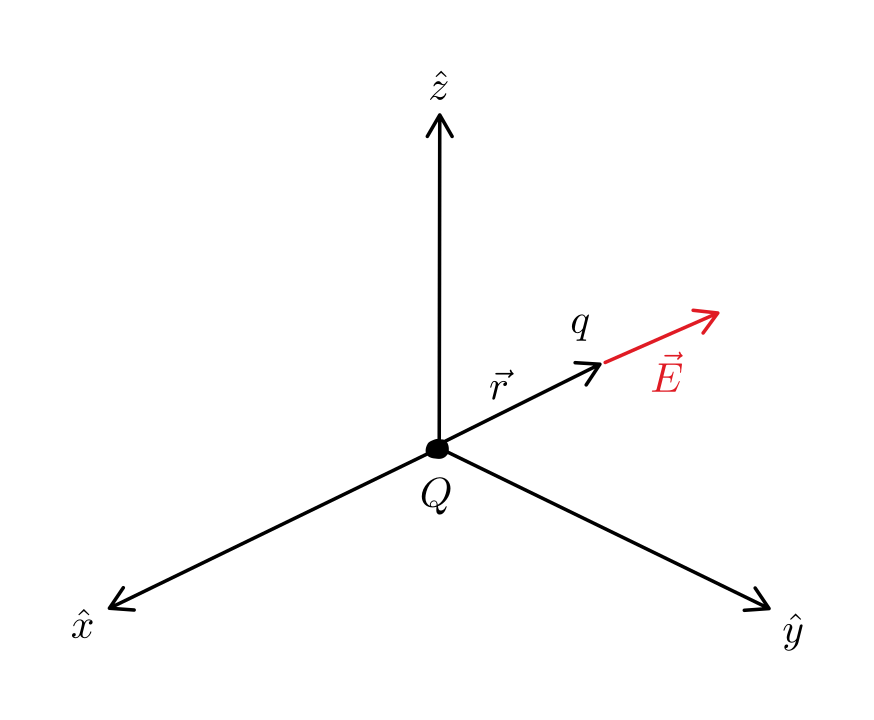
\includegraphics[width=0.6\textwidth]{campo_elettrostatico_def}
    \caption{Campo elettrostatico}
  \end{figure}
\end{definition}
\begin{definition}
  Il campo di un sistema discreto di \( n \) cariche \( q_1, q_2, \ldots, q_n \) è definito
  come:
  \[
    \vec{E} \left( \vec{r} \right) = \frac{1}{4 \pi \varepsilon_0} \sum_{i=1}^{n}
    \frac{q_i}{r_i^2} \cdot \hat{r}_i \quad \left[ \frac{N}{C} \right]
  \] 
  per il \textbf{principio di sovrapposizione}.
  \begin{figure}[H]
    \centering
    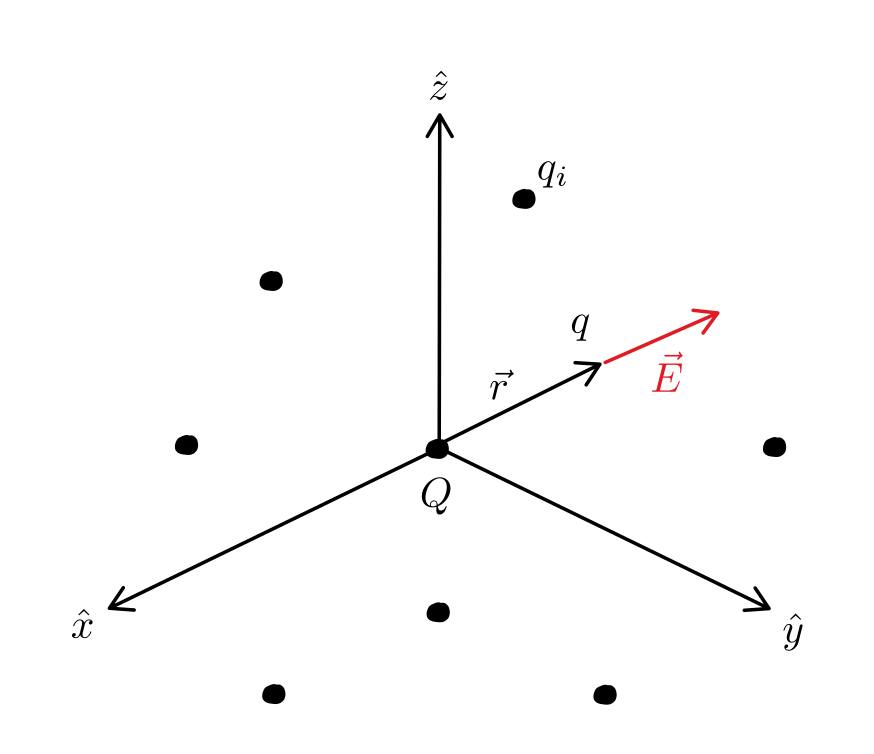
\includegraphics[width=0.6\textwidth]{campo_elettrostatico_def_piu_cariche}
    \caption{Campo elettrostatico con più cariche}
  \end{figure}
\end{definition}

\vspace{1em}
\noindent
\begin{define}
  Il \textbf{lavoro elementare} è definito come:
  \[
    dL = \vec{F} \cdot \vec{dl}
  \] 
  dove \( \vec{dl} \) è il vettore spostamento.
  \begin{itemize}
    \item Il lavoro non dipende dal percorso, ma solo dai punti di inizio e fine.
    \item Il lavoro in un percorso chiuso è nullo:
      \[
        \oint \vec{dl} = 0
      \] 
    \item Esiste una funzione di stato \( U \) tale che il lavoro per andare da \( A \) 
      a \( B \) è uguale al negativo del lavoro per andare da \( B \) a \( A \):
      \[
        \exists U \;|\; L_{AB} = - \Delta U
      \] 
      dove \( U \) è l'\textbf{energia potenziale}.
  \end{itemize}
\end{define}

\subsection{Energia potenziale elettrostatica}
La \textbf{forza elettrostatica} \( \vec{F}_{\text{el}} \) è una forza 
\textbf{conservativa}, cioè il lavoro per spostare una carica da un punto \( A \) a un 
punto \( B \) è indipendente dal percorso e dipende solo dai punti di inizio e fine.

Per calcolare il lavoro per spostare una carica \( q \) da un punto \( A \) a un punto \( B \)
si usa la seguente formula:
\[
  \begin{aligned}
    L_{AB} &= \int_{A}^{B} \vec{dL} = \int_{\text{curva}} \frac{1}{4 \pi \varepsilon_0}
    \frac{Qq}{r^2} \cdot \underbrace{\hat{r} \cdot \vec{dl}}_{dr}\\
           &= \frac{Qq}{4 \pi \varepsilon_0} \int_{r_A}^{r_B} \frac{dr}{r^2}\\
           &= \frac{Qq}{4 \pi \varepsilon_0} \left( - \frac{1}{r} \right) \Big|_{r_A}^{r_B}\\
           &= \frac{Qq}{4 \pi \varepsilon_0} \left( - \frac{1}{r_B} + \frac{1}{r_A} \right)\\
           &= - \Delta U
  \end{aligned}
\] 
dove \( U \) è l'\textbf{energia potenziale elettrostatica}:
\[
  U = \frac{Qq}{4 \pi \varepsilon_0} \cdot \frac{1}{r} + \text{costante} \quad [J]
\] 
\begin{figure}[H]
  \centering
  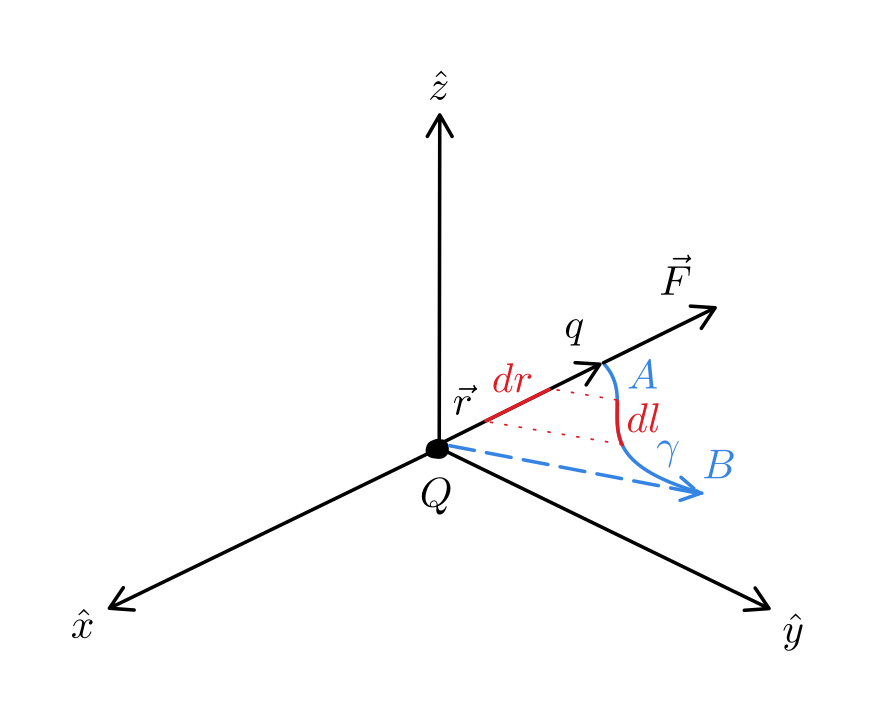
\includegraphics[width=0.7\textwidth]{energia_potenziale}
  \caption{Energia potenziale}
\end{figure}

\vspace{1em}
\noindent
Se poniamo l'energia all'infinito uguale a 0, allora \( U \) è il lavoro che fa il
campo (la forza elettrostatica) per allontanare una particella all'infinito, cioè per
distruggere il sistema:
\[
  U_{- \infty} = 0 \to U = \frac{Qq}{4 \pi \varepsilon_0 r} = - \left( U_{\infty} - U_r \right) 
\] 
\begin{itemize}
  \item Con cariche uguali l'energia è positiva perchè la forza è repulsiva e si allontana
    la carica verso l'infinito.
  \item Con cariche opposte l'energia è negativa perchè la forza è attrattiva e si avvicina
    la carica, allontanandosi dall'infinito.
\end{itemize}

\subsection{(Campo) Potenziale elettrostatico}
Dalla forza abbiamo definito l'equivalente, ma sottoforma di campo:
\begin{figure}[H]
  \centering
  \begin{tikzpicture}
    \node (f) {$\vec{F}$};
    \node[right=of f] (e) {$\vec{E} = \frac{\vec{F}}{q}$};

    \draw[->] (f) -- (e);
  \end{tikzpicture}
\end{figure}
\noindent
Si può definire un campo anche per l'energia potenziale:
\begin{figure}[H]
  \centering
  \begin{tikzpicture}
    \node (f) {$\vec{F}$};
    \node[right=of f] (e) {$\vec{E}$};
    \node[below=of f] (u) {$\Delta U$} 
      node at (u.south) [below,align=center,scale=0.7] {Energia\\elettrostatica};
    \node[below=of e] (v) {$\Delta V$} 
      node at (v.south) [below,align=center,scale=0.7] {Campo\\potenziale};


    \draw[->] (f) -- (e);
    \draw[->] (u) -- (v);
    \draw[->] (f) -- (u);
    \draw[->,dashed] (e) -- (v);
  \end{tikzpicture}
\end{figure}

\begin{definition}
  Il campo potenziale è definita come la differenza di energia di una carica \( q \) 
  unitaria:
  \[
    V(F) := \Delta V_{AB} = \frac{\Delta U}{q} \quad \left[ V \right]
  \] 
  L'unità di misura è il Volt.

  \vspace{1em}
  \noindent
  Quindi come \( \Delta U_{AB} = - \int_A^B \vec{F} \; dl \), così si avrà:
  \[
    \Delta V_{AB} = V_B - V_A = - \int_{\underset{\gamma}{A}}^B \vec{E} \; dl \quad \left[ V \right]
  \] 
  Di conseguenza il lavoro sulla carica \( q \) è:
  \[
    L_q = - q \Delta V \quad \left[ J \right]
  \] 
\end{definition}

\subsubsection{Calcolo del potenziale}
\( V(\vec{r}) \) è un campo definito a meno di una costante (come l'energia), ma si
sceglie un punto di riferimento (uno \textbf{zero}) che chiamiamo ad esempio \( \vec{r}_0 \)
e poniamo \( V(\vec{r}_0) = V_0 \). Successivamente si calcola il potenziale come
\( V(\vec{r}) - V(\vec{r}_0)\):
\[
\begin{cases}
  V(\vec{r_0}) = V_0 \to = 0\\
  V(\vec{r}) - V_0 = - \int_{\vec{r}_0}^{\vec{r}} \vec{E} \; dl
\end{cases}
\] 
Si calcola quindi il campo prendendo come punto di riferimento il punto \( \vec{r}_0 \) 

\subsubsection{Potenziale della carica puntiforme}
Ricordando la definizione di campo elettrostatico:
\[
  \vec{E} = \frac{Q}{4 \pi \varepsilon_0} \cdot \frac{\hat{r}}{r^2}
\] 
Il potenziale si calcola come:
\[
  \begin{aligned}
    V(\vec{r}) - V_0 &= - \int_{\vec{r}_0}^{\vec{r}} \vec{E} \; dl \\
                     &= - \int_{\vec{r}_0}^{\vec{r}} \frac{Q}{4 \pi \varepsilon_0}
                     \cdot \frac{\hat{r}}{r^2} \cdot  dl \\
                     &= - \frac{Q}{4 \pi \varepsilon_0} \int_{r_0}^{r} \frac{dr}{r^2} \\
                     &= \frac{Q}{4 \pi \varepsilon_0 r} -
                     \frac{Q}{4 \pi \varepsilon_0 r_0} \quad \left[ V \right]
  \end{aligned}
\] 
dove \( r_0 \) è un punto di riferimento e \( V_0 \) è il potenziale in quel punto.

Si può prendere \( r_0 = \infty \), quindi \( V_\infty = 0 \) e si ottiene:
\[
  V(\vec{r}) = \frac{Q}{4 \pi \varepsilon_0 r} \quad \left[ V \right]
\] 

\subsubsection{Potenziale di più cariche}
Consideriamo un insieme di cariche discrete \( \{q_i\}_N \) vale il \textbf{principio
di sovrapposizione} anche per il potenziale ed esso è definito tramite il campo.
Gli operatori somma e integrale commutano e quindi si ottiene:
\[
  V_{\text{tot}} = \sum V_i
\] 
dove:
\[
  V_i = \frac{q_i}{4 \pi \varepsilon_0 |\vec{r} - \vec{r}_i|}
\] 
e quindi:
\[
  V_{\text{tot}}(\vec{r}) = \frac{1}{4 \pi \varepsilon_0} \sum \frac{q_i}{|\vec{r}-\vec{r}_i|}
\] 
\begin{figure}[H]
  \centering
  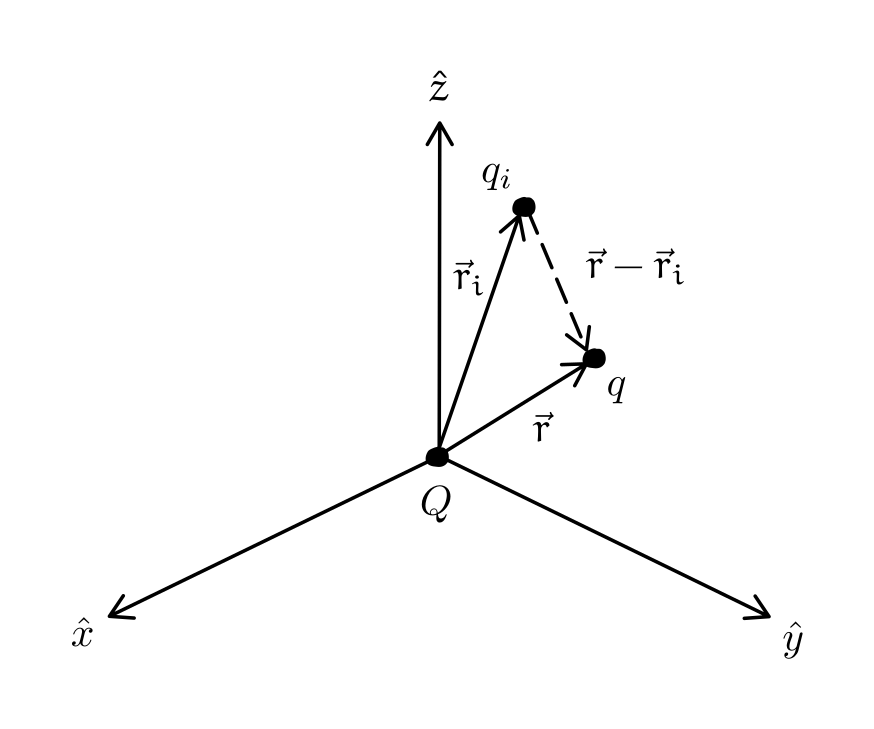
\includegraphics[width=0.6\textwidth]{potenziale_piu_cariche}
  \caption{Potenziale di più cariche}
\end{figure}
\noindent
In questo modo spostando l'origine degli assi il potenziale non cambia.

\vspace{1em}
\noindent
Se si avesse un volume tutte le sommatorie diventerebbero integrali:
\[
  V_{\text{tot}}(\vec{r}) = \frac{1}{4 \pi \varepsilon_0} \int \frac{dq}{|\vec{r} - \vec{r}_i|}
\] 

Abbiamo quindi che:
\begin{figure}[H]
  \centering
  \begin{tikzpicture}
    \node (f) {$\vec{F}$};
    \node[right=1.32cm of f] (e) {$\vec{E} = \frac{\vec{F}}{q_{\text{test}}}$};
    \node[below=of f] (u) {$\Delta U$} 
      node at (u.south) [below,align=center,scale=0.7] {Energia\\elettrostatica};
    \node[right=of u] (v) {$\Delta V = \frac{\Delta U}{q_{\text{test}}}$} 
      node at (v.south) [below,align=center,scale=0.7] {Campo\\potenziale};

    \node[below=1.1cm of u] (lu) {$L_q = - \Delta U$};
    \node[below=of v] (lv) {$L_q = -q \Delta V$};


    \draw[->] (f) -- (e);
    \draw[->] (u) -- (v);
    \draw[->] (f) -- (u) node[midway,left,scale=0.7] {conservativo};
    \draw[->] (e) -- (v) node[midway,right,scale=0.7] {conservativo};
    \draw[->] (lu) -- (lv);
  \end{tikzpicture}
\end{figure}
\noindent
La circuitazione in un percorso chiuso è nulla:
\begin{figure}[H]
  \[
    \oint_{\Gamma} \vec{E} \cdot dl = 0
  \] 
  \caption{Equazione di Maxwell}
\end{figure}
quindi \( \vec{E} \) è \textbf{conservativo}.

\subsection{Linee di campo}
Sono linee tangenti al campo elettrostatico \( \vec{E} \) in ogni punto e dirette
nel verso del campo. Hanno le seguenti caratteristiche:
\begin{itemize}
  \item Sono continue, quindi non si interrompono mai
  \item Escono dalle cariche positive e entrano nelle cariche negative
  \item Sono linee aperte, cioè non si chiudono mai

  \item In una carica positiva puntiforme sono radiali
    \begin{figure}[H]
      \centering
      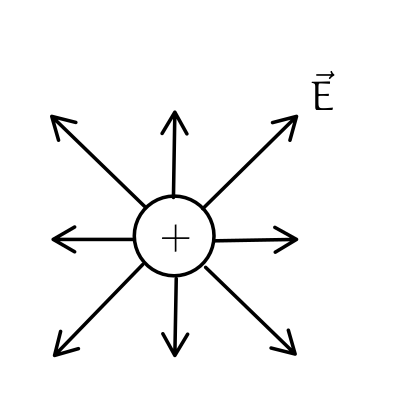
\includegraphics[width=0.3\textwidth]{linee_campo_positivo}
      \caption{Linee di campo su una carica positiva}
    \end{figure}

  \item In una carica negativa puntiforme sono radiali e entrano nella carica
    \begin{figure}[H]
      \centering
      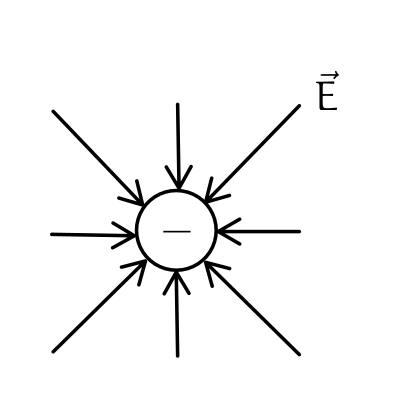
\includegraphics[width=0.3\textwidth]{linee_campo_negativo}
      \caption{Linee di campo su una carica negativa}
    \end{figure}

  \item Le cariche sono l'origine delle linee di campo, se si hanno delle linee chiuse
    vuol dire che non c'è una sorgente

  \item Le linee di campo non si intersecano mai
\end{itemize}

\subsection{Superfici equipotenziali}
Sono luoghi di punti (superficie bidimensionale) a potenziale costante:
\[
  V(\vec{r}) = \text{costante} \to \Delta V = 0 \to L = 0 \quad \text{sulla superficie}
\] 
Se il lavoro è nullo, allora la forza è perpendicolare alla superficie \( \vec{F} \perp \vec{dl} \).
Quindi le superfici equipotenziali sono perpendicolari al campo elettrico perchè:
\[
  \vec{F} = q \vec{E} \to \vec{F} \perp \vec{E}
\] 
Quindi si nota che per una carica puntiforme la superficie equipotenziale è una sfera.
Il campo elettrico punta sempre verso potenziali minori perchè il lavoro è positivo:
\begin{figure}[H]
  \centering
  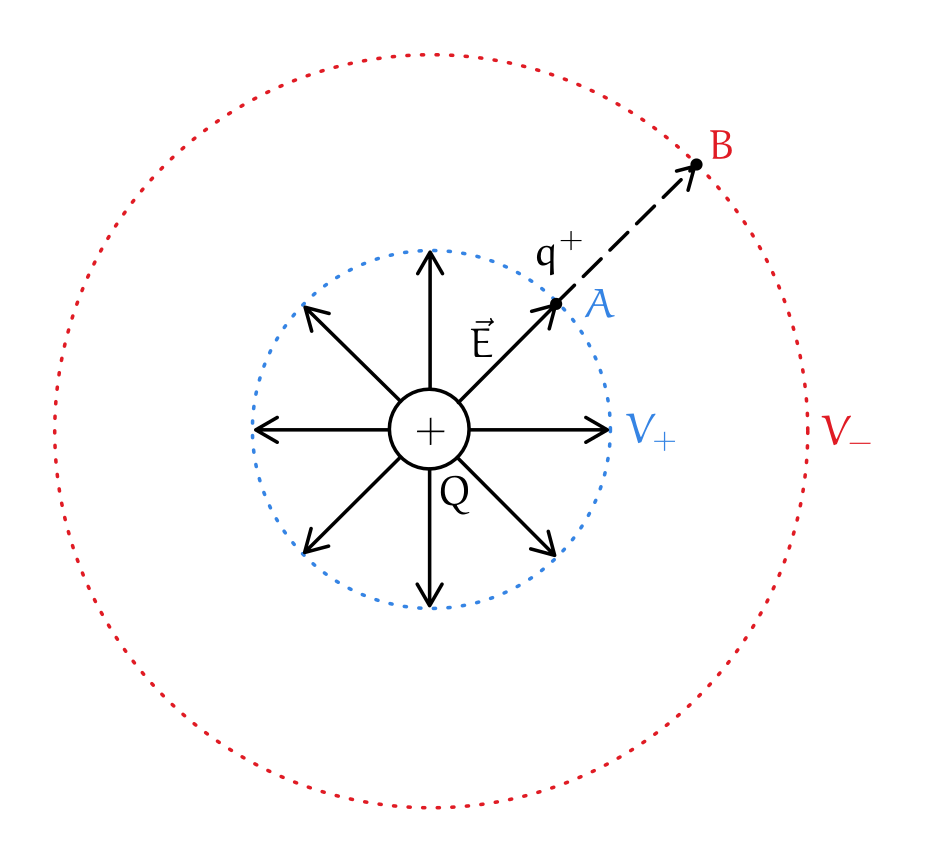
\includegraphics[width=0.8\textwidth]{superfici_equipotenziali}
  \caption{Superfici equipotenziali}
\end{figure}
\[
  L = -q^+ \left( V_B - V_A \right) > 0 \quad \text{con } V_B < V_A
\] 

\subsection{Teorema di Gauss}
Si può calcolare il campo elettrostatico \( \vec{E} \) di un'entità più complicata, come
ad esempio un filo, un cilindro ecc..., che presentano \textbf{situazioni di simmetria}.
Questo calcolo non viene fatto direttamente tramite integrali, ma tramite il \textbf{teorema
di Gauss}. Le simmetrie che analizziamo sono:
\begin{itemize}
  \item \textbf{Simmetria sfericha}: Un sistema \textbf{isotropo}, cioè che non varia in
    base alla direzione. Ad esempio una sfera, una carica puntiforme oppure un
    condensatore sferico.

  \item \textbf{Simmetria cilindrica}: Un sistema che non varia in base alla rotazione 
    intorno ad un asse. Ad esempio un cilindro \textbf{indefinito} (di lunghezza non 
    definita) oppure un filo.

  \item \textbf{Simmetria rispetto ad un piano}: Un sistema che non varia in base alla 
    traslazione lungo un piano.
\end{itemize}
Tutte queste sono geometrie in cui sono distribuite cariche e avranno una certa densità
di carica:
\begin{itemize}
  \item Carica puntiforme \( q \; \left[ C \right] \)
  \item Densità lineare \( \lambda \; \left[ \frac{C}{m} \right] \) per una linea
  \item Densità superficiale \( \sigma \; \left[ \frac{C}{m^2} \right] \) per una superficie
  \item Densità volumetrica \( \rho \; \left[ \frac{C}{m^3} \right] \) per un volume
\end{itemize}

\vspace{1em}
\noindent
\textbf{Osservazione}: Moltiplicare un campo per una superficie equivale a calcolare un
\textbf{flusso}, cioè contare le linee di campo per la superficie ortogonale. Se prendiamo
un campo di una carica puntiforme notiamo che al variare della distanza \( \vec{r} \) 
il valore del campo varia. Se invece moltiplichiamo il campo per la superficie di una 
sfera, si ottiene un flusso che è costante e non dipende da \( \vec{r} \):
\[
  \vec{E} = \frac{q \hat{r}}{4 \pi \varepsilon_0 r^2}
\] 
\[
  \vec{E} \cdot 4 \pi r^2 = \frac{q \hat{r}}{\cancel{4 \pi} \varepsilon_0 \cancel{r^2}}
  \cdot \cancel{4 \pi r^2} = \frac{q}{\varepsilon_0} \cdot \hat{r}
\] 

\begin{define}[Angolo piano]
  L'angolo solido \( d \alpha \) è definito come un elemento di linea \( dl \) di 
  circonferenza diviso per il raggio:
  \begin{figure}[H]
    \centering
    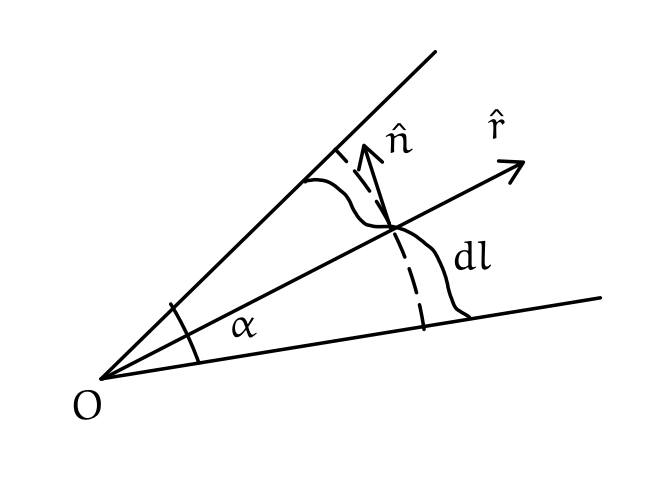
\includegraphics[width=0.4\textwidth]{angolo_piano}
    \caption{Angolo piano}
  \end{figure}
  \[
    d \alpha = \frac{\vec{dl} \cdot \hat{n} \cdot \hat{r}}{r}
  \] 
\end{define}
\begin{define}[Angolo solido]
  L'angolo solido \( d \Omega \) è definito come un elemento di superficie \( dS \) diviso
  per il raggio al quadrato:
  \begin{figure}[H]
    \centering
    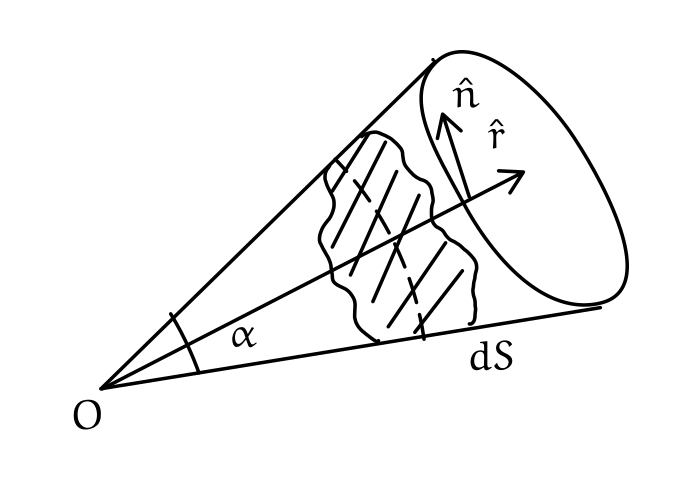
\includegraphics[width=0.4\textwidth]{angolo_solido}
    \caption{Angolo solido}
  \end{figure}
  \[
    d \Omega = \frac{dS \cdot \hat{n} \cdot \hat{r}}{r^2}
  \]
  
\end{define}

\subsubsection{Flusso del campo \texorpdfstring{\( \vec{E} \)}{E}}
Consideriamo una superficie con concavità verso il basso definita come la sua orientazione
\( \hat{n} \) (normale) e la sua area \( dS \).
\begin{figure}[H]
  \centering
  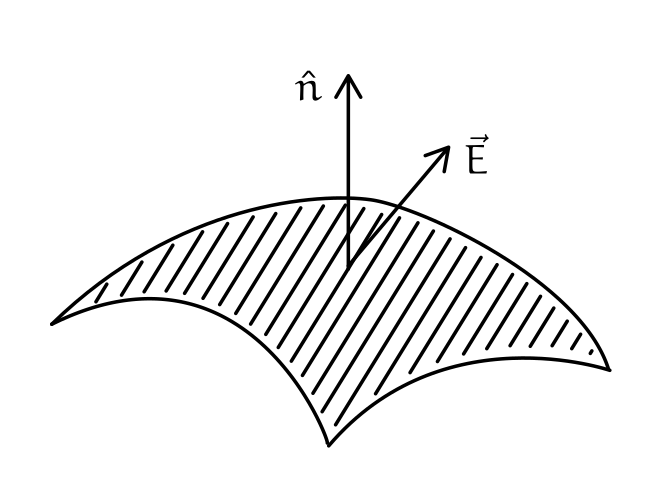
\includegraphics[width=0.6\textwidth]{superficie}
  \[
    d\vec{S} = \hat{n} \cdot dS
  \] 
  \caption{Superficie}
\end{figure}
\begin{definition}[Flusso elementare]
  Il flusso elementare \( d \Phi \) è definito come il prodotto scalare tra il campo
  e la superficie:
  \[
    d \Phi = \vec{E} \cdot d \vec{S} \quad \left[ V \cdot m \right]
  \] 

  \vspace{1em}
  \noindent
  Il flusso di una superficie si ottiene integrando:
  \[
    \Phi = \oint \vec{E} \cdot d \vec{S}
  \] 
  \begin{figure}[H]
    \centering
    \setkeys{Gin}{width=\linewidth}
    \begin{subfigure}{0.3\textwidth}
      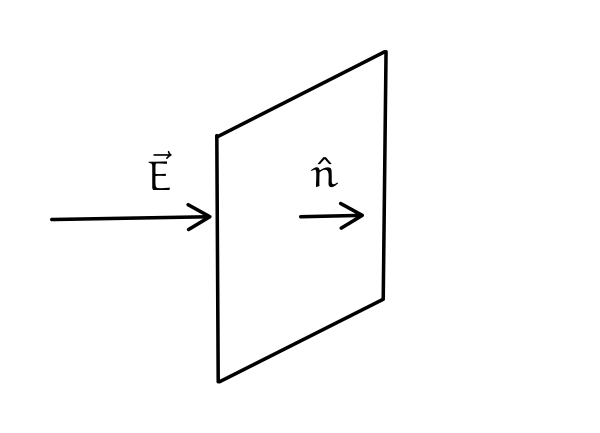
\includegraphics{flusso_positivo}
      \[
        d \Phi > 0
      \] 
      \caption{Flusso positivo}
    \end{subfigure}
    \hfil
    \begin{subfigure}{0.3\textwidth}
      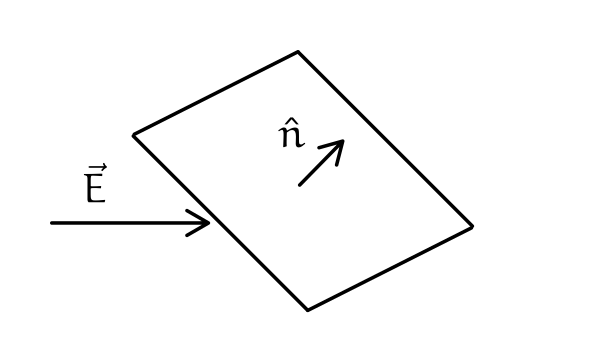
\includegraphics{flusso_generico}
      \[
       \Phi = \vec{E} \cdot \vec{S} \cos \theta
      \] 
      \caption{Flusso generico}
    \end{subfigure}
    \hfil
    \begin{subfigure}{0.3\textwidth}
      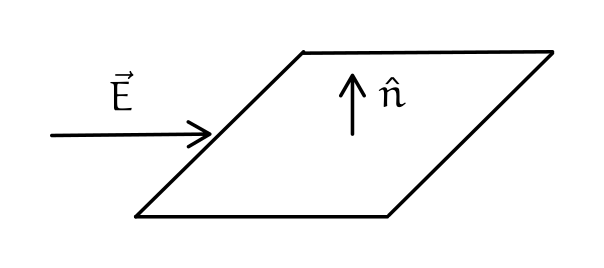
\includegraphics{flusso_nullo}
      \[
        \Phi = \vec{E} \cdot \vec{S} = 0
      \] 
      \caption{Flusso nullo}
    \end{subfigure}
    \caption{Esempi di flusso}
  \end{figure}
\end{definition}

\begin{example}
  Consideriamo una carica puntiforme \( q \) e una superficie \( dS \) 
  \begin{figure}[H]
    \centering
    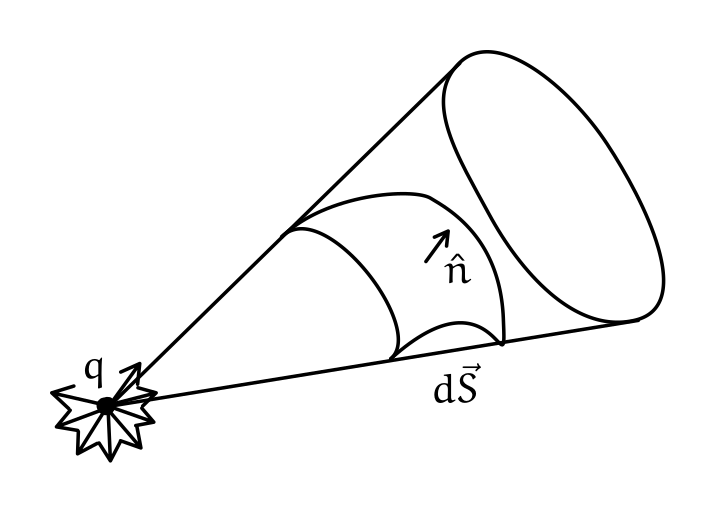
\includegraphics[width=0.5\linewidth]{flusso_puntiforme}
    \caption{Flusso di una carica puntiforme}
  \end{figure}
  Il flusso del campo elettrostatico è:
  \[
    d \Phi = \left( \vec{E} \cdot d\vec{S} \right) = \frac{q}{4 \pi \varepsilon_0} 
    \underbrace{\frac{\hat{r}}{r^2} \cdot d\vec{S}}_{d \Omega} = \frac{q}{4 \pi \varepsilon_0}
    d \Omega
  \] 
  Osserviamo che il flusso dipende solo da \( d \Omega \), cioè dall'angolo solido,
  e non dalla distanza \( r \) della superficie dalla carica.
\end{example}
\begin{example}
  Consideriamo una superficie chiusa:
  \begin{figure}[H]
    \centering
    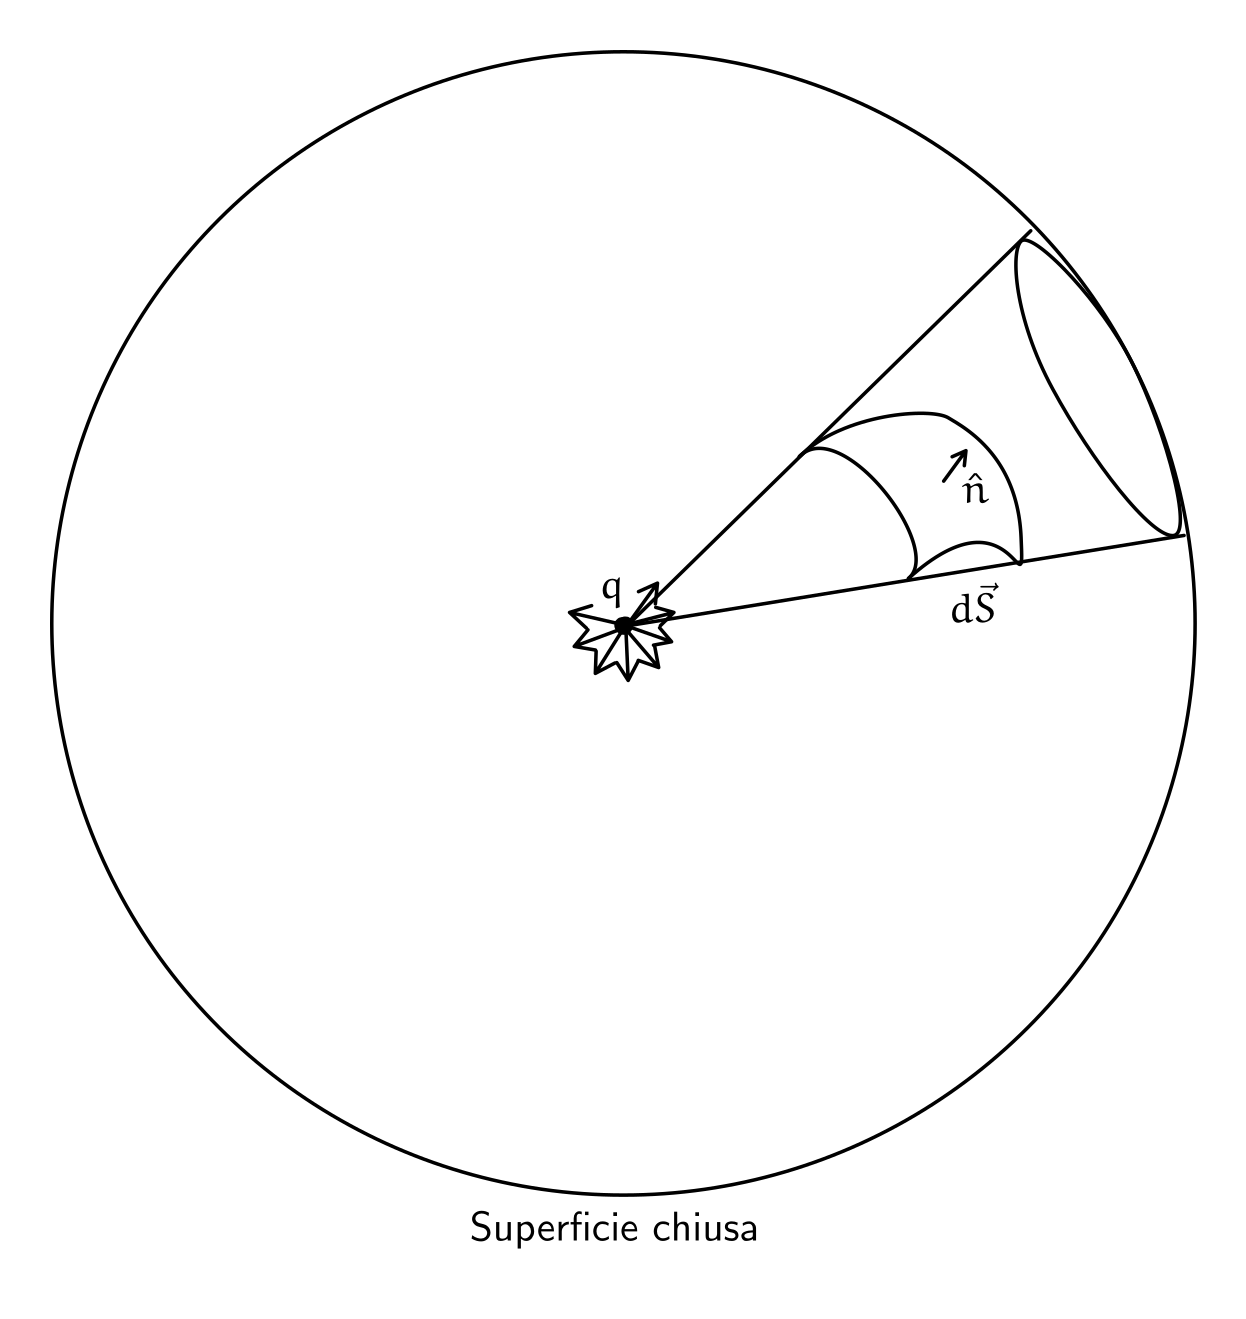
\includegraphics[width=0.7\linewidth]{flusso_superficie_chiusa}
    \caption{Flusso di una superficie chiusa}
  \end{figure}
  il flusso del campo elettrostatico è:
  \[
    \Phi = \oint \frac{q}{4 \pi \varepsilon_0} d \Omega = \frac{q}{4 \pi \varepsilon_0}
    \underbrace{\oint d \Omega}_{= 4 \pi} = \frac{q}{\varepsilon_0}
  \] 
  L'integrale su una superficie chiusa dell'angolo piano è uguale a \( 2 \pi  \),
  quindi l'integrale su una superficie chiusa dell'angolo solido è uguale a \( 4 \pi \).
\end{example}
Il flusso quindi non dipende dalla superficie. Questa è la dimostrazione del teorema
di Gauss.

\begin{theorem}[Teorema di Gauss]
  Il flusso \( \Phi(\vec{E}) \) del campo elettrico \( \vec{E} \) attraverso una
  superficie chiusa \textbf{qualsiasi} \( S \) è uguale alla somma delle cariche interne alla superficie
  diviso \( \varepsilon_0 \):
  \[
    \Phi (\vec{E}) = \underset{\text{superficie chiusa QUALUNQUE}}{\oint} \vec{E} \cdot d \vec{S} = \frac{Q_{\text{interne}}}{\varepsilon_0}
  \] 
  Le cariche esterne non contano perchè quando esse entrano nella superficie, ad un
  certo punto escono, quindi il flusso è nullo. Se all'interno della superficie c'è
  una sorgente (quindi cariche interne) esse non entrano mai perchè sono già dentro,
  quindi escono e il flusso è positivo.
\end{theorem}

\subsection{Applicazione del teorema di Gauss}
Siccome il teorema di Gauss dice che il flusso non dipende dalla superficie si prende
una superficie particolarmente simmetrica chiamata \textbf{superficie di Gauss} che
rende facilmente calcolabile il flusso, grazie al campo costante su tutta la superficie.
Per calcolare il campo \( \vec{E} \) siccome esso è costante e parallelo alla normale
(grazie alla superficie scelta) si può tirare fuori dall'integrale per ottenere un
prodotto tra l'incognita \( \vec{E} \) e un integrale geometrico.
\begin{figure}[H]
  \[
    \Phi (\vec{E}) = \vec{E} \cdot \oint_{\text{Sup}} d \vec{S} =
    \frac{Q_{\text{Interne}}}{\varepsilon_0}
  \] 
  \caption{Equazione di Maxwell}
\end{figure}
\subsubsection{Simmetria sferica}
Le caratteristiche necessarie sono:
\begin{itemize}
  \item Distribuzione di carica con simmetria sferica. Potrebbe essere una:
    \begin{itemize}
      \item Carica di volume \( \rho \)
        \begin{figure}[H]
          \centering
          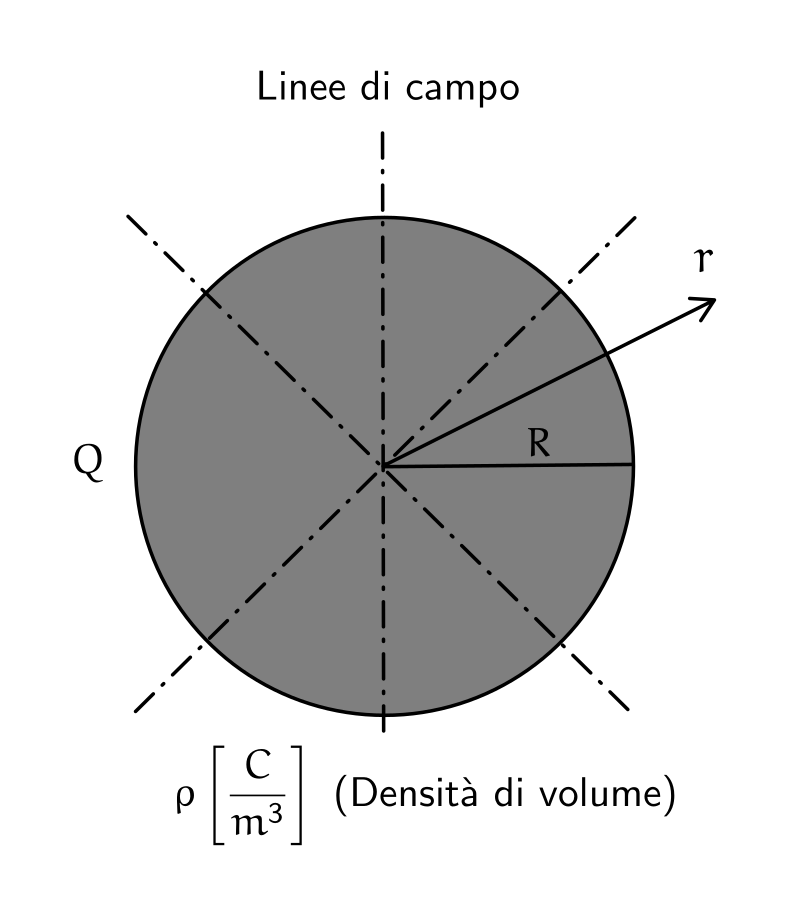
\includegraphics[width=0.5\textwidth]{simmetria_sferica_volume}
          \[
            Q = \rho \cdot \overbrace{\frac{4}{3}\pi R^3}^{\text{Volume sfera}}
            \quad \left[C\right]
          \] 
          \caption{Simmetria sferica di volume}
        \end{figure}
      \item Carica di superficie \( \sigma \)
        \begin{figure}[H]
          \centering
          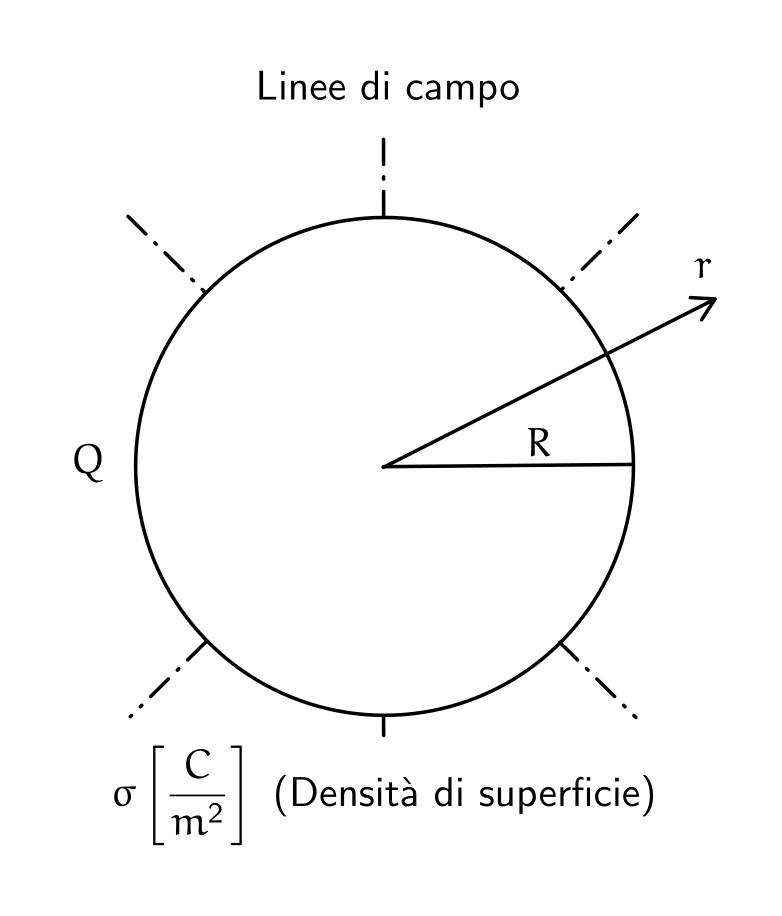
\includegraphics[width=0.5\textwidth]{simmetria_sferica_superficie}
          \[
            Q = \sigma \cdot \overbrace{4 \pi R^2}^{\text{Superficie sfera}}
            \quad \left[C\right]
          \] 
          \caption{Simmetria sferica di superficie}
        \end{figure}
    \end{itemize}
    Se la carica \( \{Q\} \) è a simmetria sferica, allora il campo \( \vec{E} \) sarà
    a simmetria sferica. Questo campo sarà \textbf{radiale} e dipenderà solo da \( \vec{r} \):
    \[
      \vec{E} = E(r) \hat{r}
    \] 
\end{itemize}

\begin{example}
  Consideriamo una carica positiva \( Q^+ \) distribuita su una superficie. L'obiettivo
  è quello di cercare una superficie di Gauss in cui il campo elettrico sia costante.
  Siccome dipende solo da \( r \) esso sarà costante solo nelle superfici sferiche \( S(r) \) 
  di raggio \( r \).
  \begin{figure}[H]
    \centering
    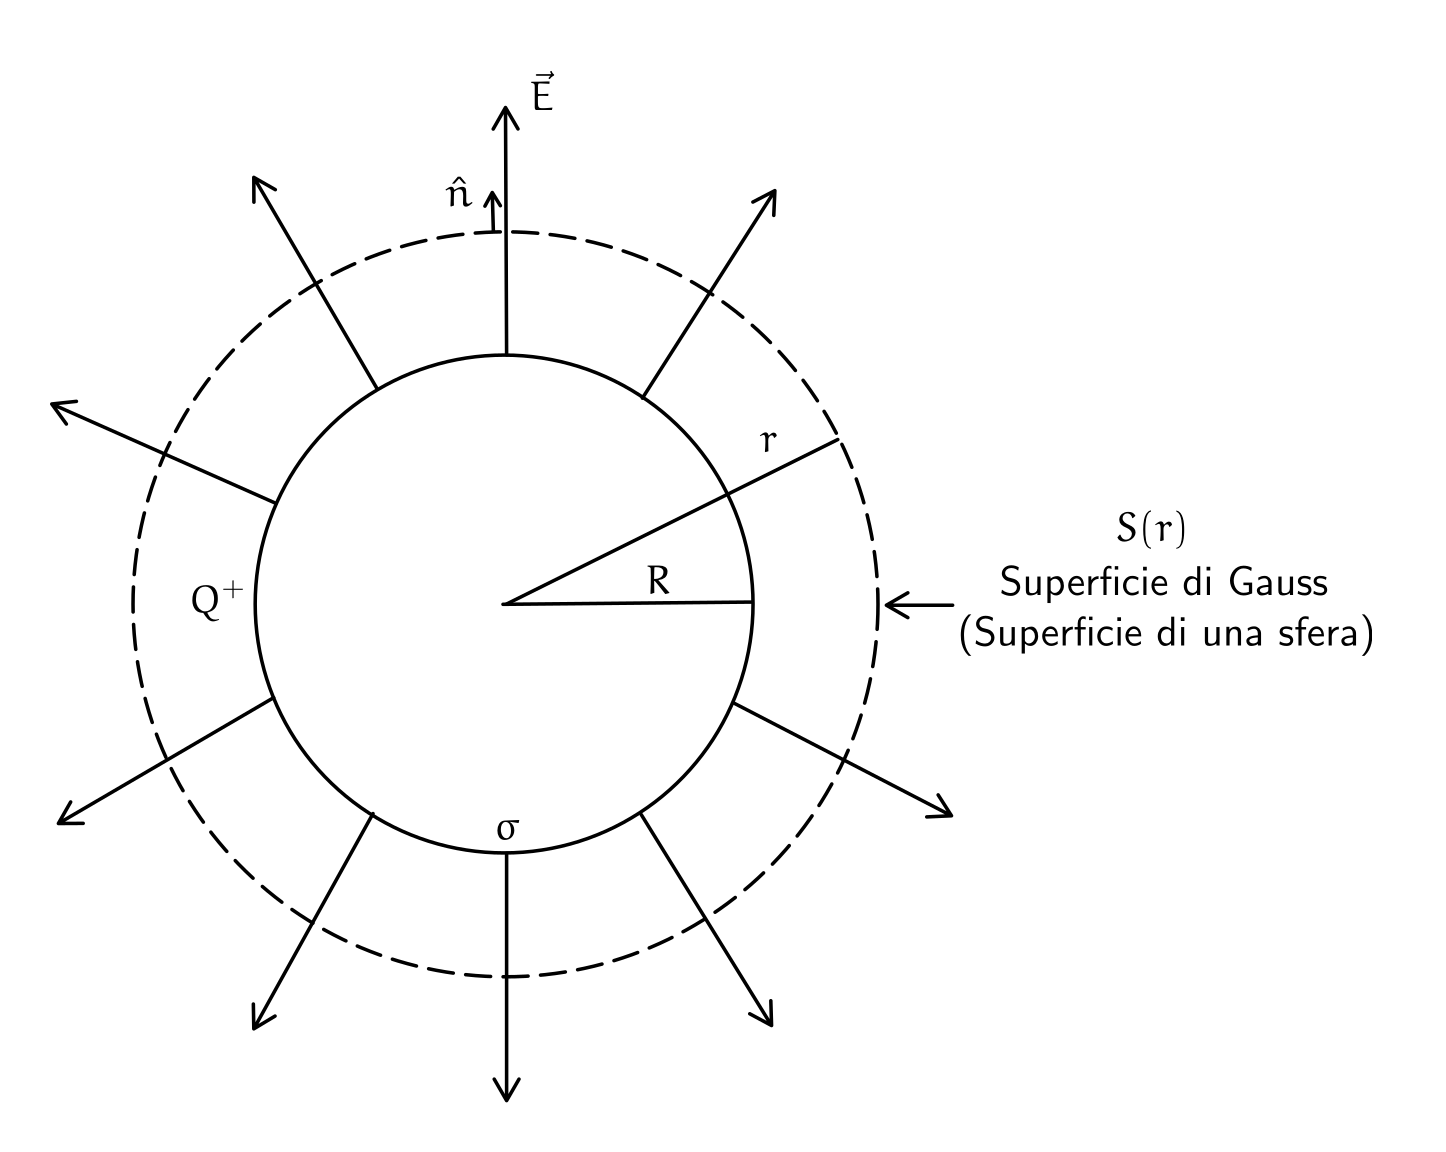
\includegraphics[width=0.9\textwidth]{carica_superficie_sferica}
    \caption{Carica distribuita su una superficie sferica}
  \end{figure}
  \[
    \begin{aligned}
      \Phi(\vec{E}) &= \oint_{S(r)} \vec{E} \cdot \hat{n} \cdot_{S(r)} dS\\
      &= \oint_{S(r)} E(r) dS\\
      &= E(r) \overbrace{\oint_{S(r)} dS}^{\text{Sup sfera}}\\
      &= E(r) \cdot 4 \pi r^2 = \frac{Q_{\text{int}}}{\varepsilon_0}
    \end{aligned}
  \]
  Dove:
  \[
    Q_{\text{int}} =
  \begin{cases}
    Q & \text{se } r \ge R \text{ (esterno)}\\
    0 & \text{se } r < R \text{ (interno)}
  \end{cases}
  \] 
  Quindi:
  \[
    E(r) = \begin{cases}
      \frac{Q}{4 \pi \varepsilon_0 r^2} & \text{se } r \ge R\\
      0 & \text{se } r < R
    \end{cases}
    \quad \left[ \frac{V}{m} \right]
  \] 
  In \( r = R \) il campo vale:
  \[
    E(R) = \frac{Q}{4 \pi \varepsilon_0 R^2} = \frac{\sigma}{\varepsilon_0}
  \] 
  Il grafico del campo elettrico è:
  \begin{figure}[H]
    \centering
    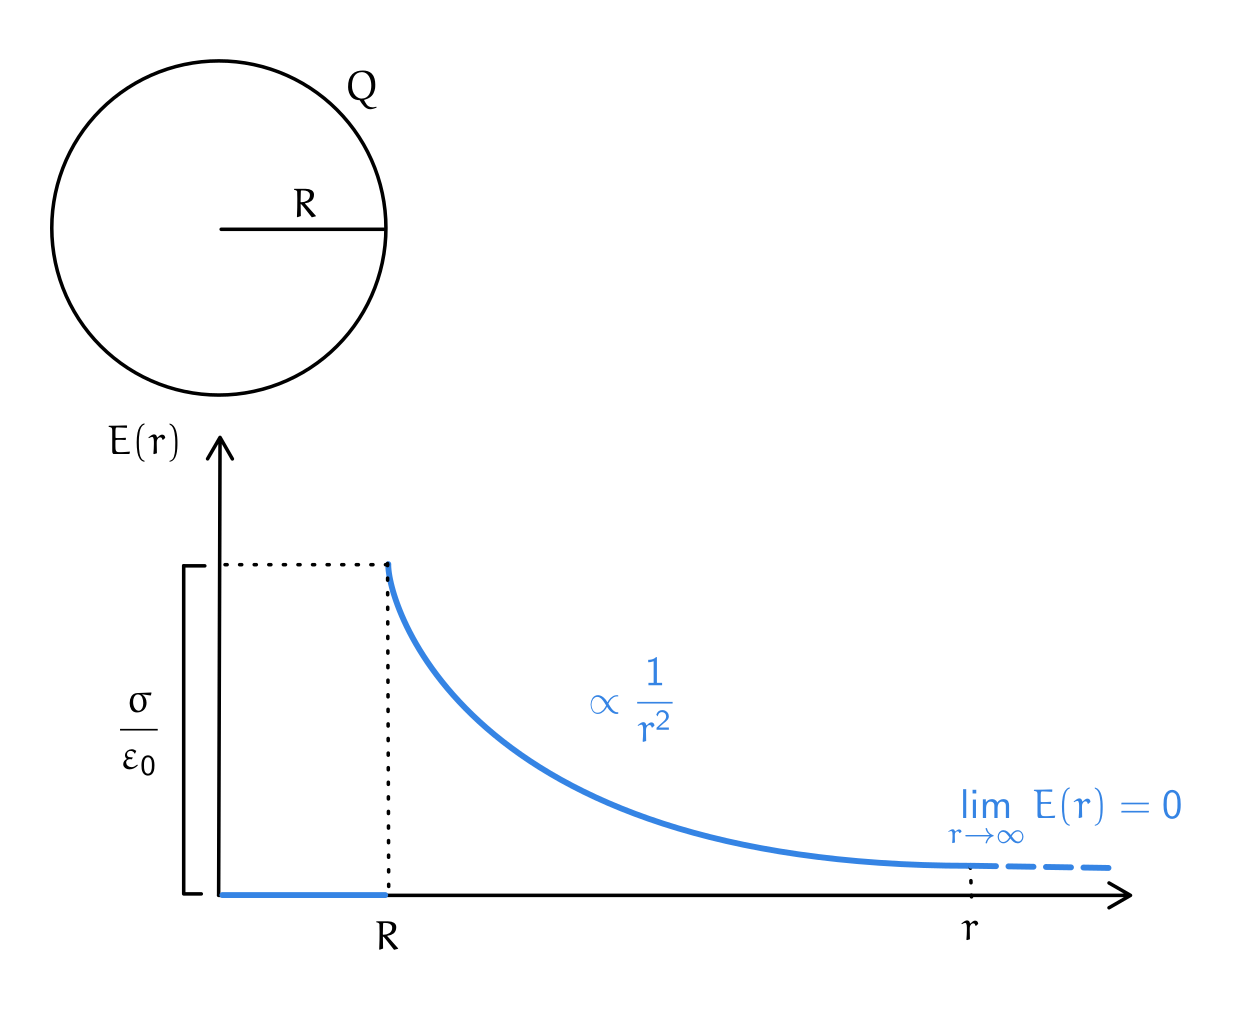
\includegraphics[width=0.9\textwidth]{grafico_superficie_sferica}
    \caption{Grafico del campo elettrico}
  \end{figure}
\end{example}
\begin{example}
  Consideriamo una carica positiva \( Q^+ \) distribuita su un volume. L'obiettivo è
  quello di cercare una superficie di Gauss in cui il campo elettrico sia costante.
  Siccome dipende solo da \( r \) esso sarà costante solo nelle sfere \( S(r) \) di raggio
  \( r \).
  \begin{figure}[H]
    \centering
    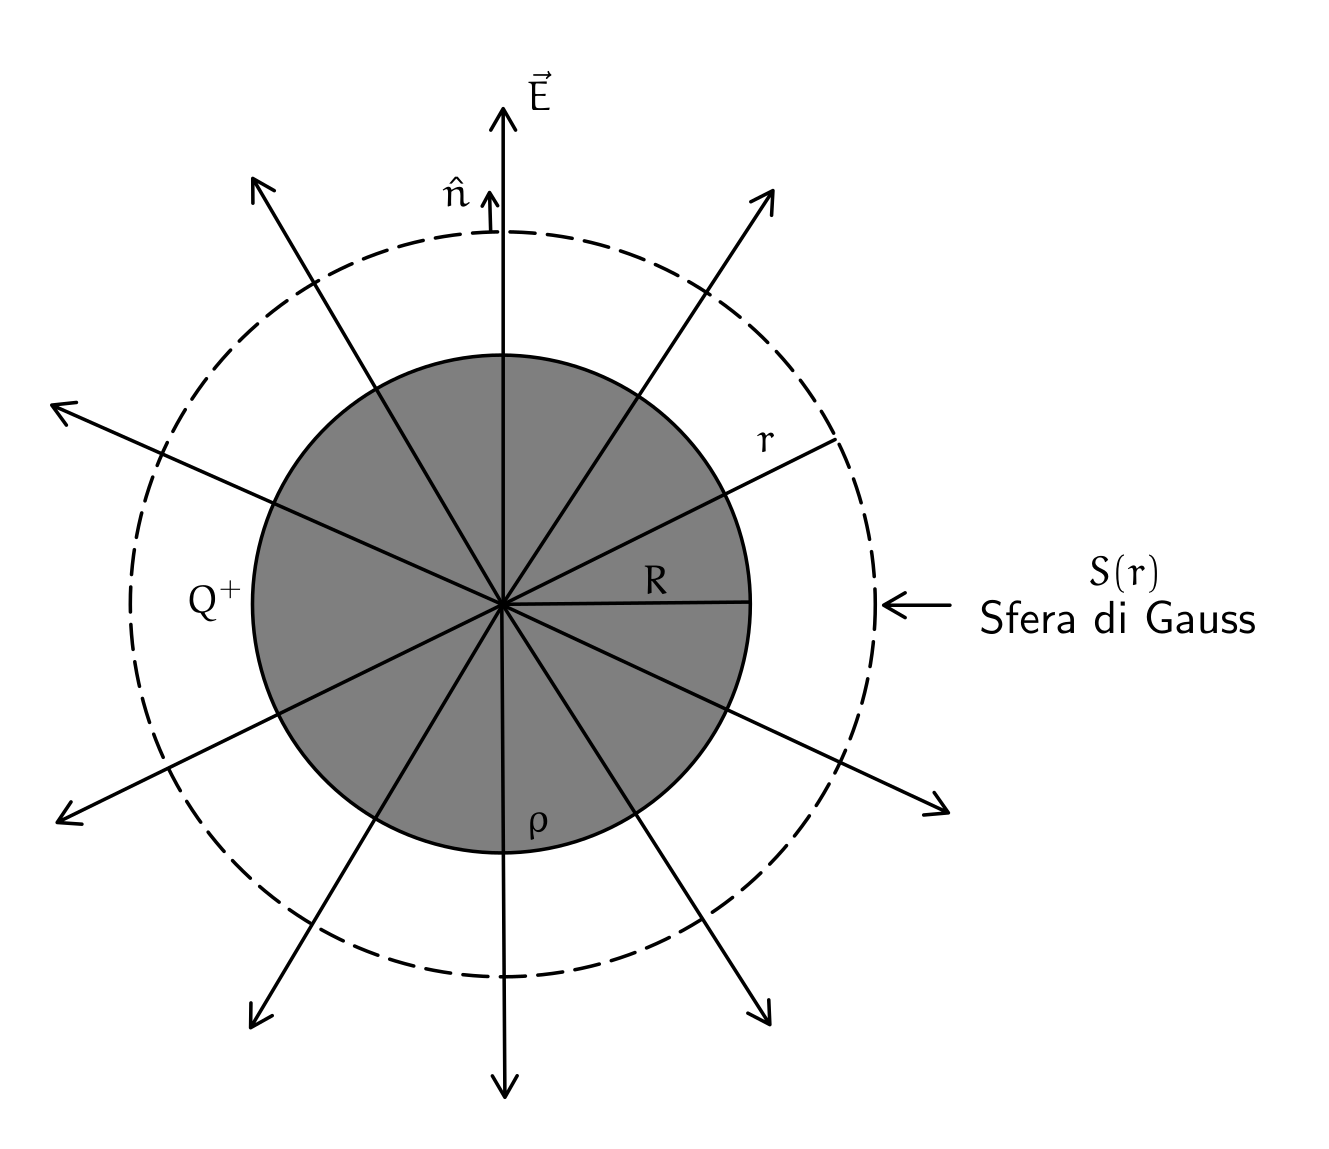
\includegraphics[width=0.9\textwidth]{carica_volume_sferico}
    \caption{Carica distribuita su un volume sferico}
  \end{figure}
  \noindent
  Siccome la sfea all'interno non è più vuota come nell'esempio precedente, ma è piena
  il valore di \( Q_{\text{int}} \) esterno rimane invariato, ma all'interno si ha:
  \[
    Q_{\text{Int}} = 
    \begin{cases}
      Q & \text{se } r \ge R\\
      \rho \cdot \frac{4}{3} \pi r^3 & \text{se } r < R
    \end{cases}
  \] 
  Quindi:
  \[
    E(r) = \begin{cases}
      \frac{Q}{4 \pi \varepsilon_0 r^2} & \text{se } r \ge R\\
      \frac{\rho}{3 \varepsilon_0} \cdot r & \text{se } r < R
    \end{cases}
    \quad \left[ \frac{V}{m} \right]
  \]
  In \( r = R \) il campo vale:
  \[
    E(R) = \frac{\frac{4}{3} \pi R^3 \rho}{4 \pi \varepsilon_0 R^2} 
    = \frac{\rho}{3 \varepsilon_0} \cdot R
  \] 
  Il grafico del campo elettrico è:
  \begin{figure}[H]
    \centering
    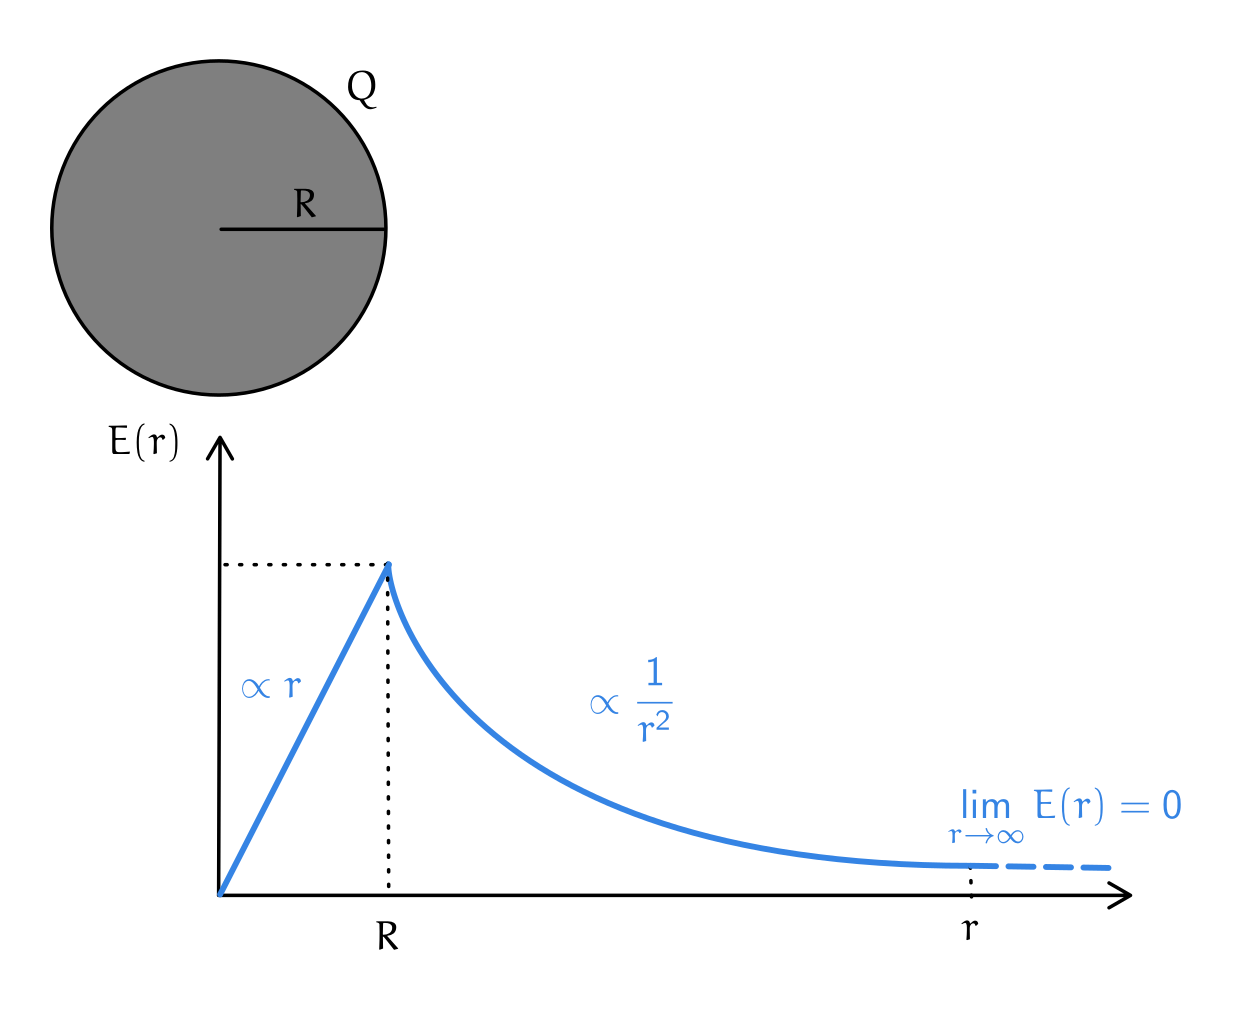
\includegraphics[width=0.9\textwidth]{grafico_volume_sferico}
  \end{figure}
\end{example}

\subsubsection{Simmetria cilindrica}
Le possibili simmetrie sono:
\begin{itemize}
  \item Filo indefinito con distribuzione di carica lineare \( \lambda \)
  \item Cilindro
    \begin{itemize}
      \item Con distribuzione di carica sulla superficie
      \item Con distribuzione di carica nel volume
    \end{itemize}
\end{itemize}
La caratteristica principale è la \textbf{simmetria attorno all'asse del sistema}.
La superficie di Gauss in cui il campo è costante è un cilindro di raggio \( r \) e
altezza \( h \).
\begin{example}
  Consideriamo una carica \( \lambda^+ \) distribuita su un filo indefinito:
  \begin{figure}[H]
    \centering
    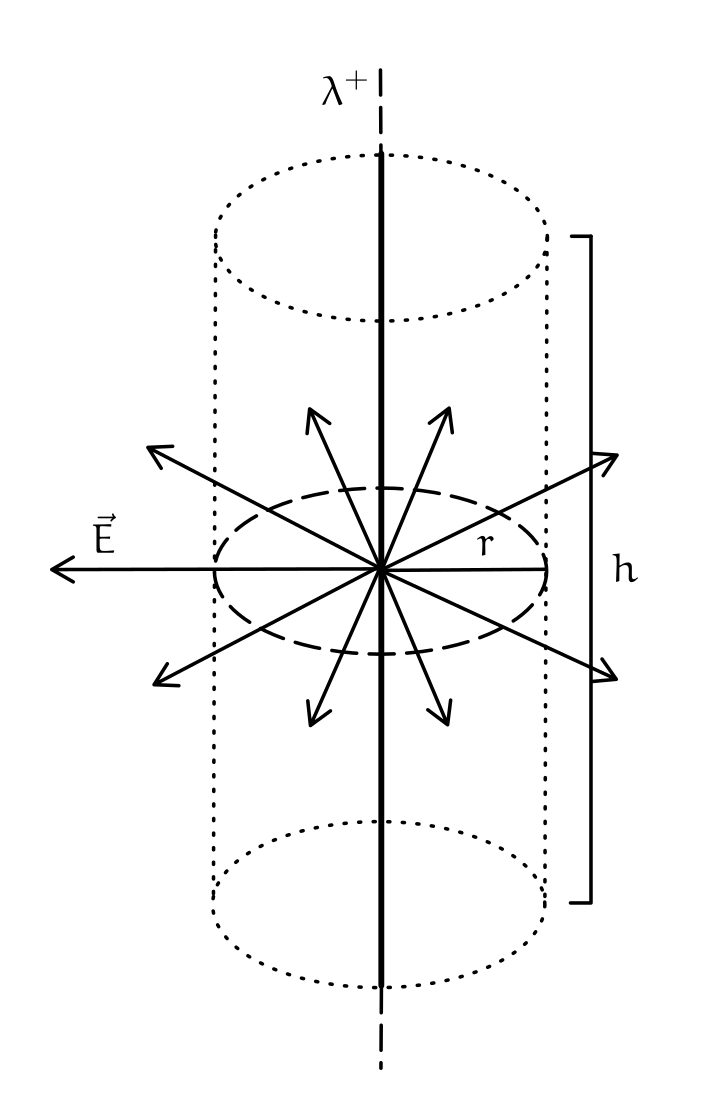
\includegraphics[width=0.5\textwidth]{carica_filo_indefinito}
    \caption{Carica distribuita su un filo indefinito}
  \end{figure}
  \noindent
  Il flusso del campo è il flusso delle basi (che essendo perpendicolari al campo radiale
  vale 0) più il flusso laterale:
  \[
    \Phi (\vec{E}) = \Phi_{\text{Basi}} + \Phi_{\text{Laterale}} = 0 + E \cdot 2 \pi r h =
    \frac{Q_{\text{Int}}}{\varepsilon_0} = \frac{\lambda h}{\varepsilon_0}
  \] 
  Quindi il campo è:
  \[
    E(r) = \frac{\lambda}{2 \pi \varepsilon_0 r}
  \] 
  Il grafico del campo elettrico è:
  \begin{figure}[H]
    \centering
    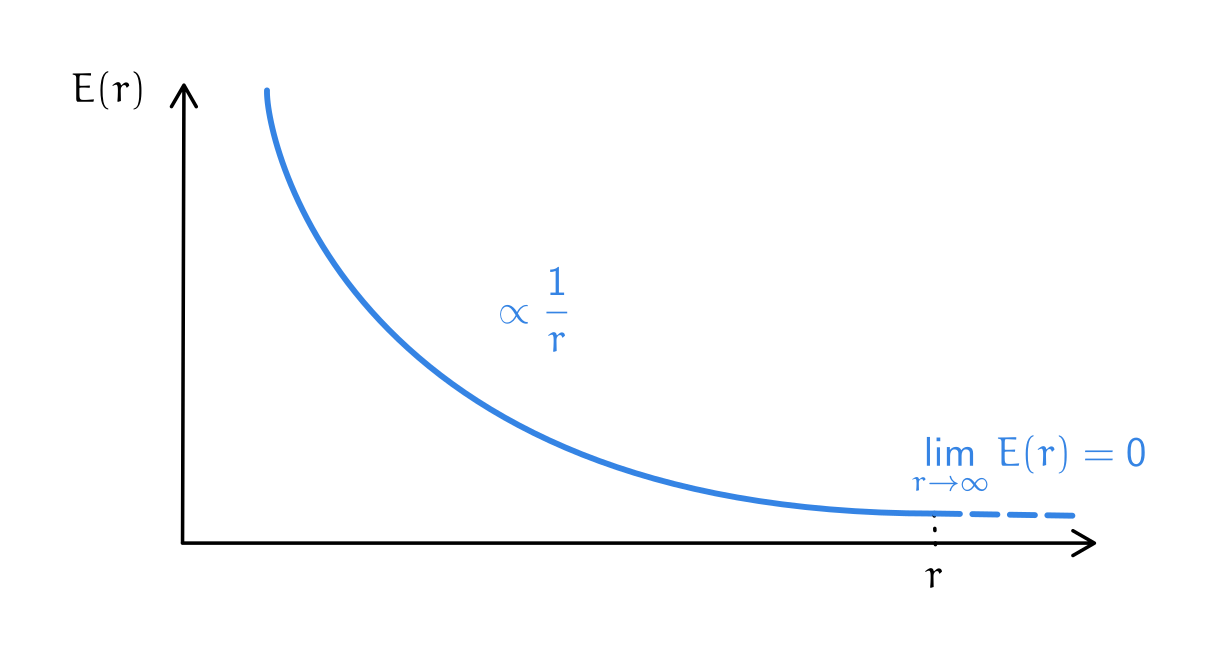
\includegraphics[width=0.9\textwidth]{grafico_filo_indefinito}
    \caption{Grafico del campo elettrico}
  \end{figure}
\end{example}
\begin{example}
  Consideriamo una carica \( \sigma^+ \) distribuita su un cilindro di raggio \( R \) e
  altezza \( h \):
  \begin{figure}[H]
    \centering
    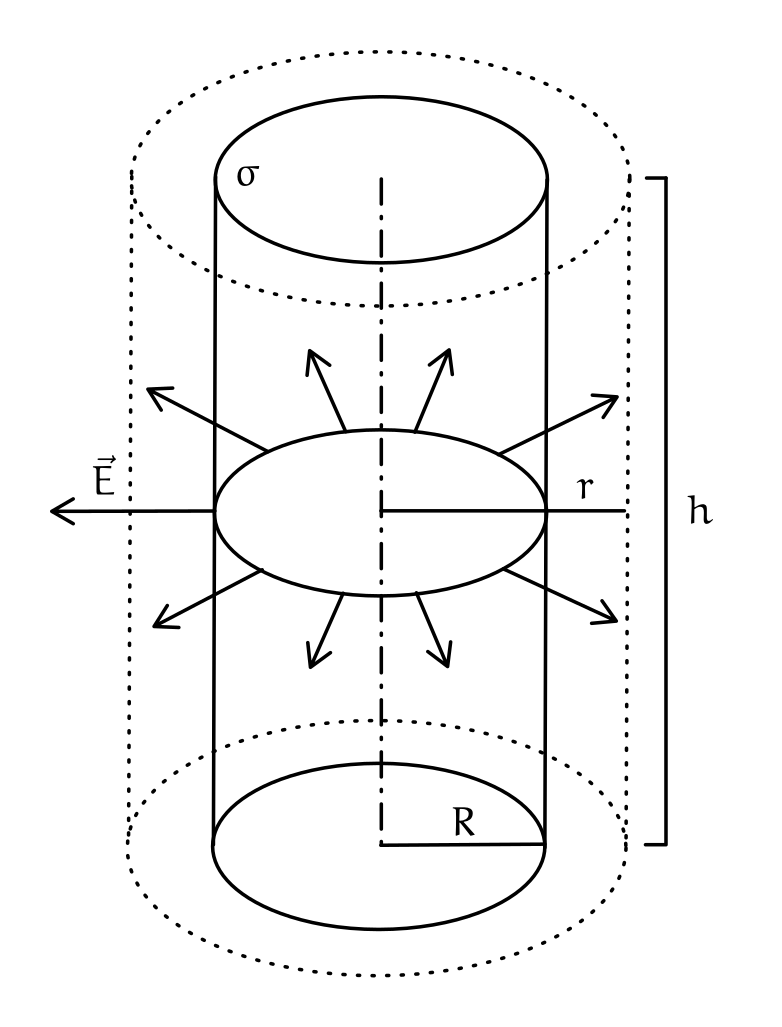
\includegraphics[width=0.5\textwidth]{carica_superficie_cilindrica}
    \caption{Carica distribuita su un cilindro di raggio \( R \) e altezza \( h \)}
  \end{figure}
  Il flusso del campo è lo stesso del caso precedente, ma con \( Q_{\text{Int}} \) diverso:
  \[
    Q_{\text{Int}} =
    \begin{cases}
      \sigma \cdot 2 \pi R h & \text{se } r \ge R\\
      0 & \text{se } r < R
    \end{cases}
  \] 
  Quindi il campo è:
  \[
    E(r) = \begin{cases}
      \frac{\sigma R}{\varepsilon_0 r} & \text{se } r \ge R\\
      0 & \text{se } r < R
    \end{cases}
  \]
  Il grafico del campo elettrico è:
  \begin{figure}[H]
    \centering
    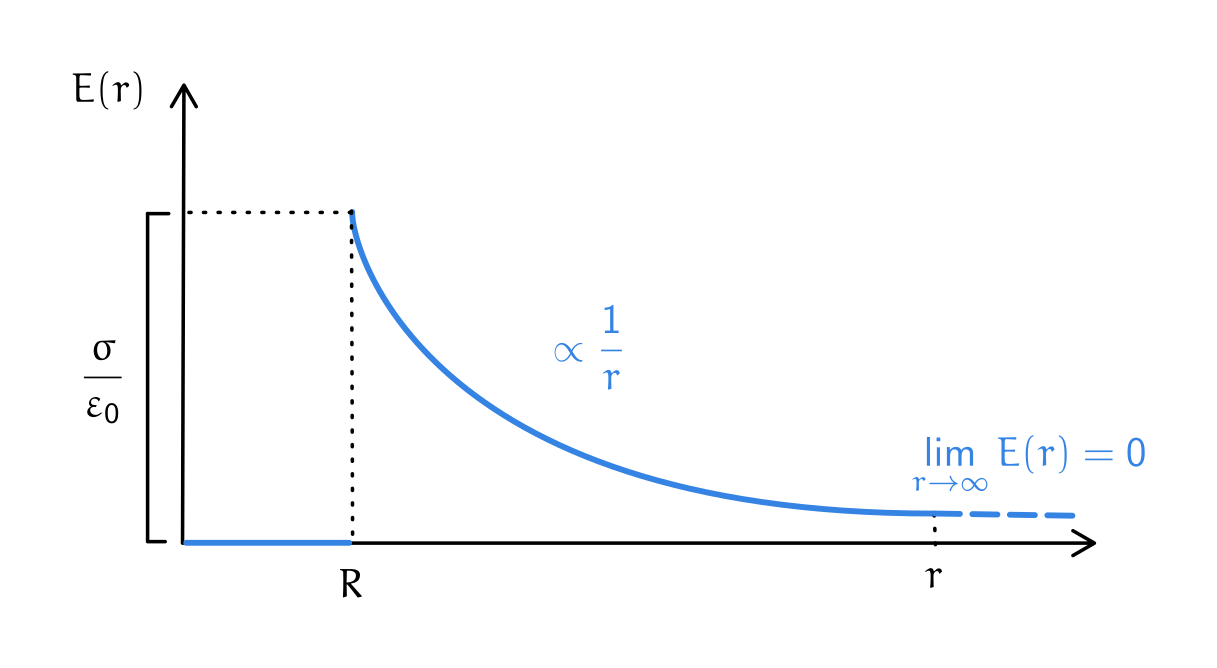
\includegraphics[width=0.9\textwidth]{grafico_superficie_cilindrica}
    \caption{Grafico del campo elettrico}
  \end{figure}
\end{example}

\subsubsection{Simmetria rispetto ad un piano indefinito}
Consideriamo un piano indefinito con una distribuzione di carica superficiale 
positiva \( \sigma^+ \; \left[ \frac{C}{m^2} \right] \). L'unico grado di libertà
è la distanza dal piano. L'elemento di campo è definito come:
\[
  d\vec{E} = \frac{dq}{4 \pi \varepsilon_0 r^2} \hat{r}
\] 
Se consideriamo un elemento di carica che agisce su un punto \( p \), allora siccome
il piano è indefinito ci sarà un elemento di carica simmetrico che genera un campo
con componente orizzontale uguale e opposto a quella dell'elemento precedente.
Di conseguenza il campo totale sarà perpendicolare al piano:
\begin{figure}[H]
  \centering
  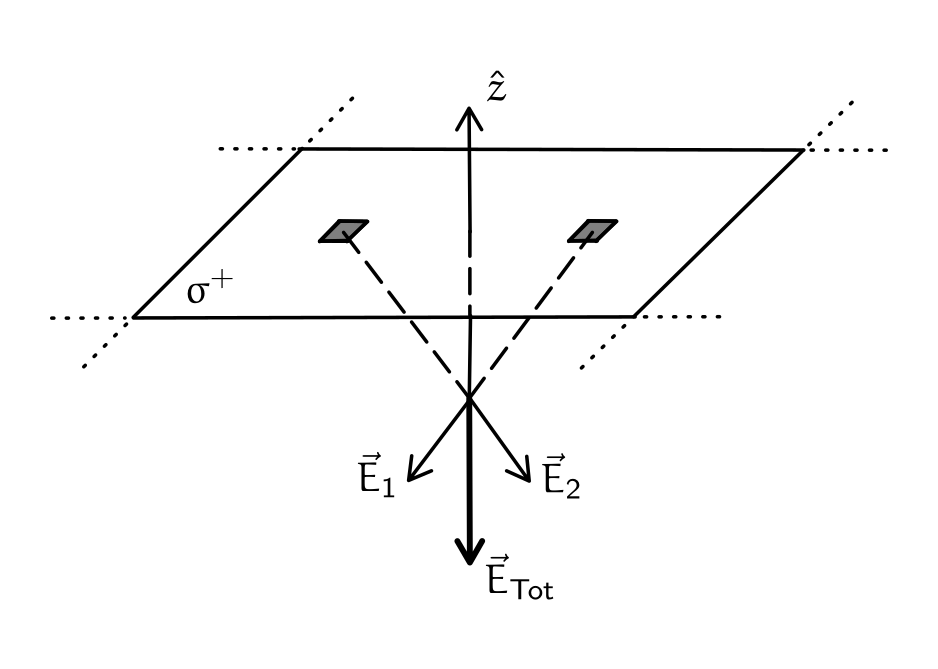
\includegraphics[width=0.7\textwidth]{carica_superficie_piano}
  \caption{Carica distribuita su un piano indefinito}
\end{figure}
\noindent
Il campo avrà questa forma:
\[
  \vec{E} = E(z) \hat{z}
\] 
La superficie di Gauss da considerare è un cilindro che si trova metà sopra e metà sotto
il piano:
\begin{figure}[H]
  \centering
  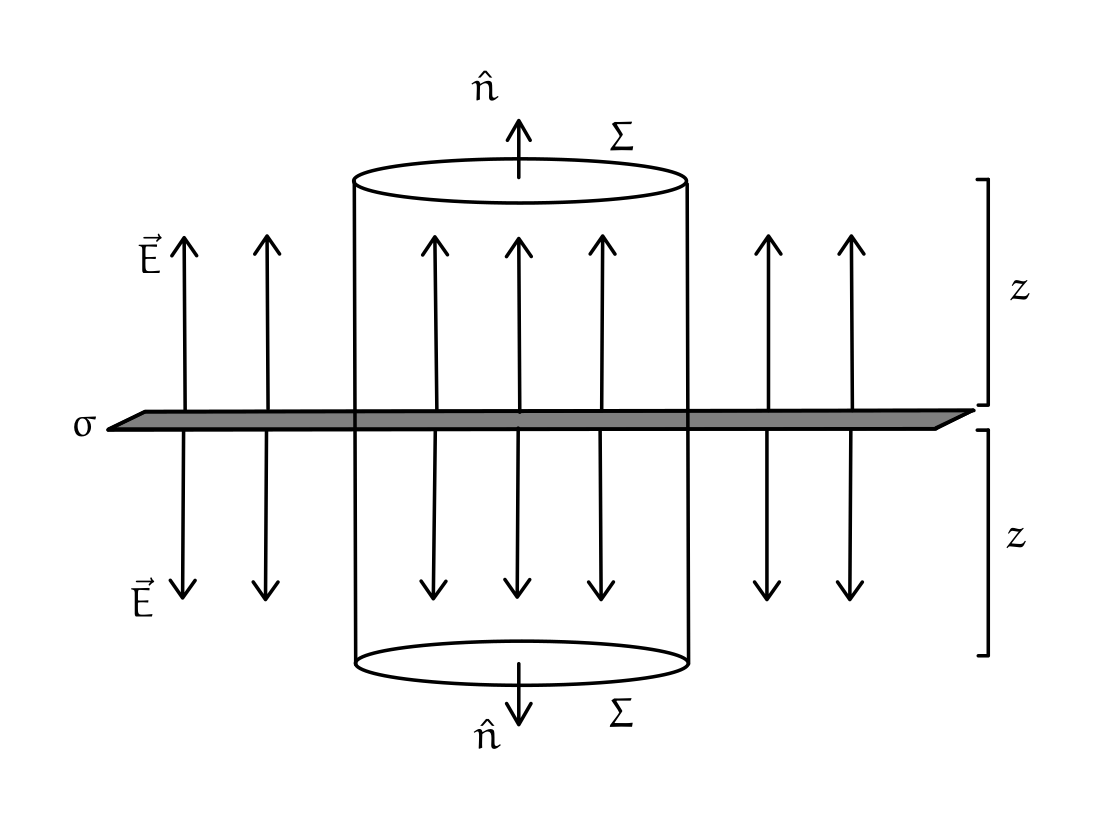
\includegraphics[width=0.8\textwidth]{superficie_gauss_piano}
  \caption{Superficie di Gauss per un piano indefinito}
\end{figure}
\noindent
Il flusso del sistema sarà il flusso delle basi più il flusso dei lati, ma il flusso
laterale sarà nullo:
\[
  \Phi = \Phi_{\text{Basi}} + \Phi_{\text{Laterale}} = 2 E(z) \cancel{\Sigma} + 0 
  = \frac{Q_{\text{Int}}}{\varepsilon_0} = \frac{\cancel{\Sigma} \sigma}{\varepsilon_0}
\] 
Quindi il campo è:
\[
  E = \frac{\sigma^\pm}{2 \varepsilon_0}
\] 
La particolarità di questo campo è che non dipende dalla distanza, quindi è un campo
costante.

\begin{example}
  Vogliamo analizzare il campo elettrico tra due piani indefiniti distanti \( h \) uno
  caricato positivamente e l'altro negativamente.
  \begin{figure}[H]
    \centering
    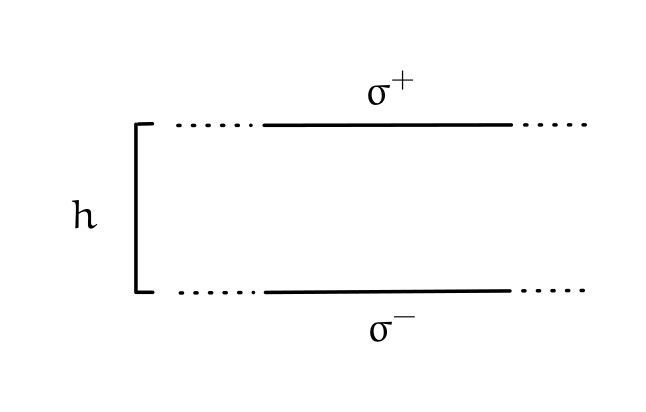
\includegraphics[width=0.5\textwidth]{carica_superficie_piano_positivo_negativo}
    \caption{Carica distribuita su due piani indefiniti}
  \end{figure}
  \noindent
  Il piano, per il principio di sovrapposizione, è uguale a:
  \[
    \sigma = \sigma ^+ + \sigma ^-
  \] 
  \begin{figure}[H]
    \centering
    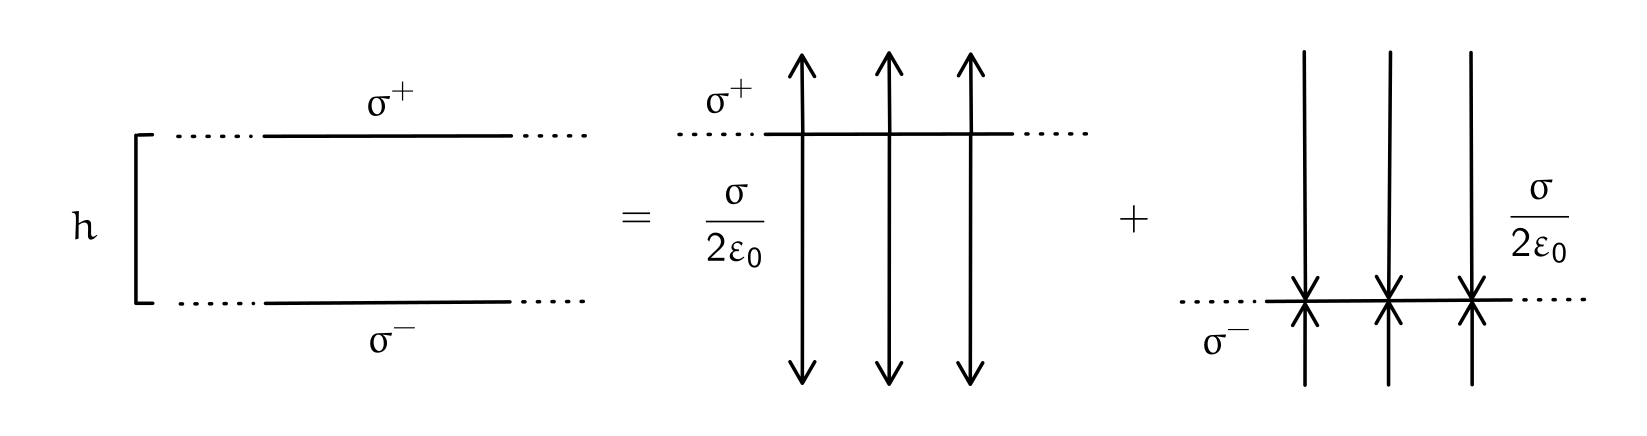
\includegraphics[width=1.\textwidth]{sovrapposizione_piano}
    \caption{Sovrapposizione di due piani}
  \end{figure}
  \noindent
  Dal teorema di Gauss abbiamo che il campo è costante e vale:
  \[
    \vec{E} = \frac{\sigma}{2 \varepsilon_0}
  \] 
  quindi:
  \begin{figure}[H]
    \centering
    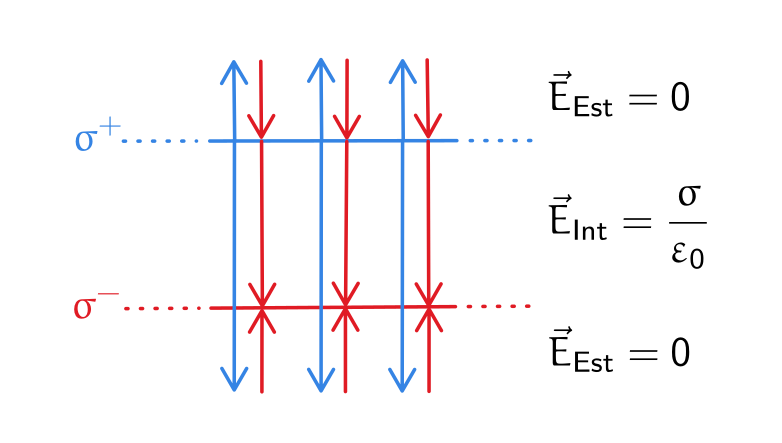
\includegraphics[width=0.7\textwidth]{sovrapposizione_piano_2}
    \caption{Risultato della sovrapposizione di due piani}
  \end{figure}
  \noindent
  Notiamo che all'esterno dei piani il campo è nullo, mentre al centro è la somma
  dei due campi con verso dal positivo al negativo.
  \[
    \vec{E} = \frac{\sigma}{2\varepsilon_0} + \frac{\sigma}{2\varepsilon_0} =
    \frac{\sigma}{\varepsilon_0}
  \] 
  Le linee di campo sono quindi:
  \begin{figure}[H]
    \centering
    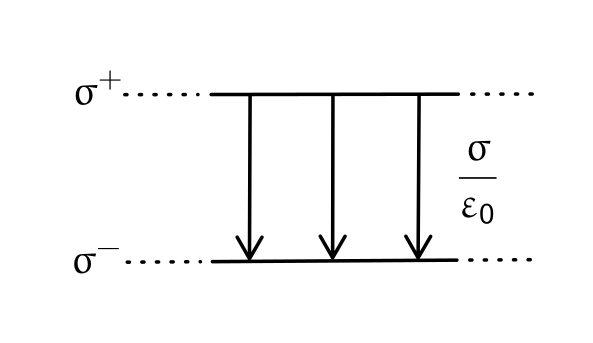
\includegraphics[width=0.5\textwidth]{linee_campo_piano}
    \caption{Linee di campo tra due piani}
  \end{figure}
\end{example}

\subsection{Elettrostatica nei conduttori}
Un materiale conduttore ha \textbf{le cariche libere di muoversi}. Se si avvicina un
campo elettrico e sulle cariche viene esercitata una forza. Per un momento ci sarà
del caos, ma poi le cariche si sposteranno fino a quando non si raggiunge l'equilibrio,
in quel momento si studia il comportamento delle cariche.

\subsubsection{Proprietà dei conduttori in equilibrio elettrostatico}
\begin{enumerate}
  \item \textbf{Prima proprietà}: Il campo totale interno in un conduttore è 0:
    \[
      E_{\text{Interno}} = 0
    \] 

    \vspace{1em}
    \noindent
    Consideriamo un conduttore immerso in un campo chiamato \textbf{campo esterno}.
    Le cariche sono libere di muoversi, quindi quelle positive andranno nella direzione
    del campo, mentre quelle negative andranno nella direzione opposta al campo.
    \begin{figure}[H]
      \centering
      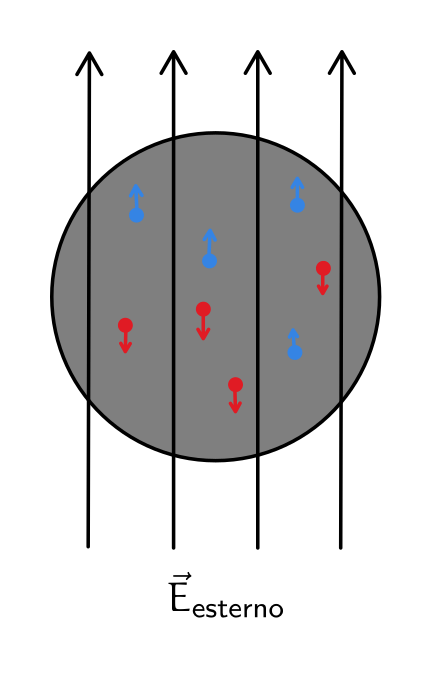
\includegraphics[width=0.4\textwidth]{conduttore_campo_esterno}
      \caption{Campo esterno in un conduttore}
    \end{figure}
    Si nota quindi una separazione di carica che creerà un \textbf{campo indotto}.
    \begin{figure}[H]
      \centering
      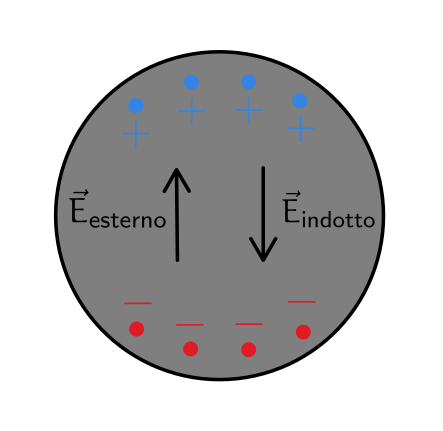
\includegraphics[width=0.4\textwidth]{conduttore_campo_indotto}
      \caption{Campo indotto in un conduttore}
    \end{figure}
    Vale il principio di sovrapposizione e quindi all'interno del conduttore si avrà
    la somma dei due campi:
    \[
      E_{\text{tot}} = E_{\text{est}} + E_{\text{ind}}
    \] 
    Ad un certo punto si raggiungerà l'equilibrio, quindi le cariche non si muovono più,
    di conseguenza il campo è nullo.

  \item \textbf{Seconda proprietà}: Siccome il campo è nullo, il potenziale è costante su
    tutto il conduttore:
    \[
      V - V_0 = - \int_{\vec{r}_0}^{\vec{r}} \cancel{\vec{E}} \cdot d\vec{l}
    \] 
    \[
      V = \text{costante}
    \] 

  \item \textbf{Terza proprietà}: Siccome il campo interno è nullo, la carica interna
    in un conduttore in equilibrio è 0 (dal teorema di Gauss) \( Q_{\text{Int}} = 0 \) :
    \[
      \oint_S \cancel{\vec{E}} \cdot d\vec{S} = \frac{Q_{\text{int}}}{\varepsilon_0} = 0 \to Q_{\text{int}} = 0
    \] 
    Quindi \textbf{le cariche si distribuiscono solo in superficie}

  \item \textbf{Quarta proprietà}: Il campo nella superficie di un conduttore è ortogonale 
    alla superficie e vale sempre:
    \[
      \vec{E}_{\text{sup}} = \frac{\sigma}{\varepsilon_0} \hat{n}
    \] 
    (Teorema di Coulomb)
\end{enumerate}
Notiamo quindi che il conduttore in equilibrio elettrostatico distorce il campo nel
seguente modo:
\begin{figure}[H]
  \centering
  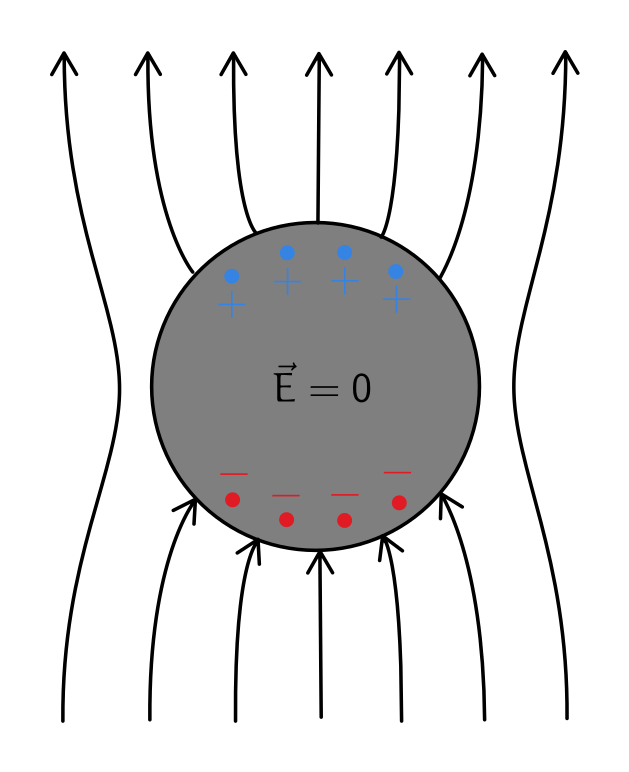
\includegraphics[width=0.5\textwidth]{conduttore_equilibrio}
  \caption{Campo in un conduttore in equilibrio}
\end{figure}

\subsubsection{Cavità in un conduttore}
La cavità non dipende dalla geometria del conduttore. Un esempio di un conduttore con
una cavità è il seguente (un guscio):
\begin{figure}[H]
  \centering
  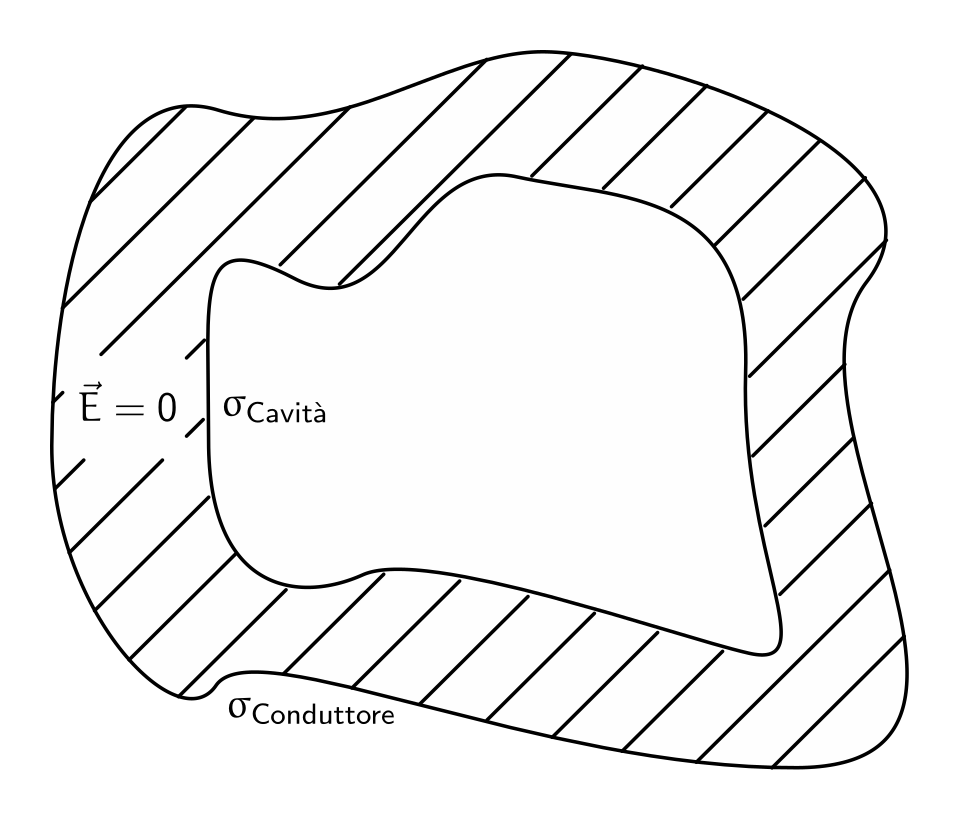
\includegraphics[width=0.6\textwidth]{conduttore_guscio}
  \caption{Conduttore con una cavità}
\end{figure}

\noindent
Carichiamo un conduttore con una cavità \textbf{vuota} con una carica \( Q \). Questa carica
si distribuirà sulla superficie del conduttore e ha le seguenti proprietà:
\begin{enumerate}
  \item La densità nella superficie della cavità è scarica:
    \[
      \sigma_{\text{Cavità}} = 0
    \] 
    quindi se si deposita una carica sul guscio, l'interno non può essere caricato
    
  \item Il campo all'interno della cavità è nullo:
    \[
      E_{\text{Cavità}} = 0
    \] 
    \textbf{Dimostrazione}: Per il teorema di Gauss posiziono una superficie di Gauss
    all'interno del conduttore, quindi:
    \begin{figure}[H]
      \centering
      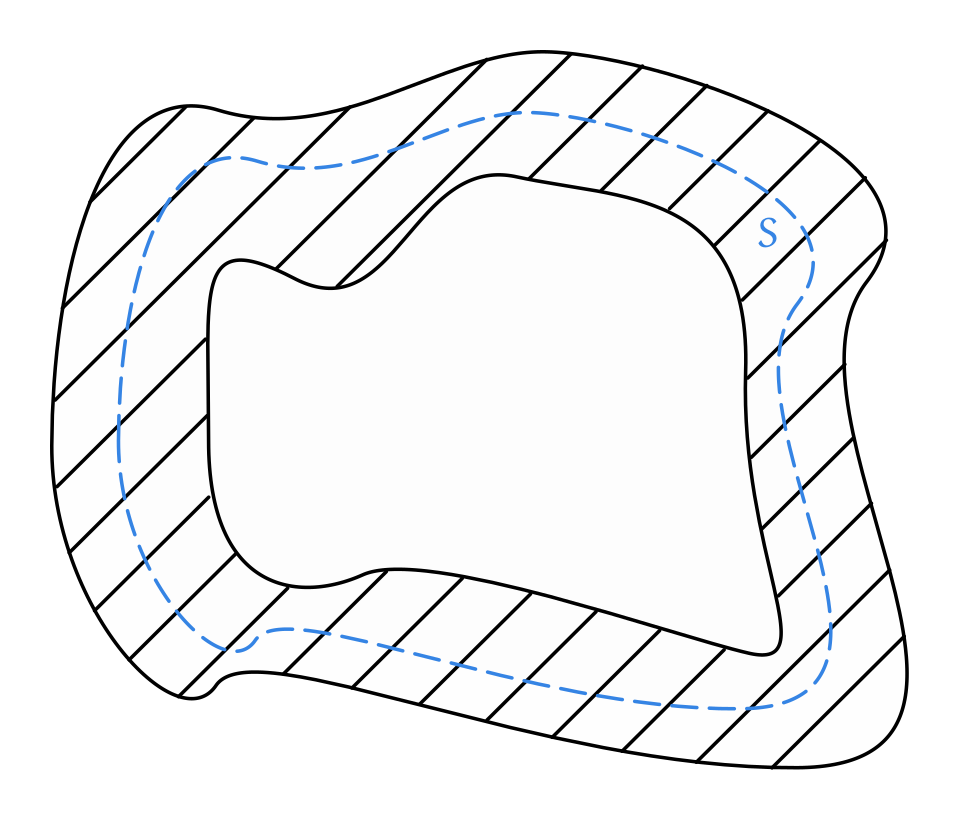
\includegraphics[width=0.6\textwidth]{superficie_gauss_conduttore_cavita}
      \caption{Superficie di Gauss in un conduttore con cavità}
    \end{figure}
    \[
      \oint_S \vec{E} \cdot d\vec{S} = \frac{Q_{\text{int \textbf{totale}}}}{\varepsilon_0}
    \] 
    Il campo vale 0 perchè la superficie di Gauss si trova all'interno del conduttore,
    quindi:
    \[
      \oint_S \vec{E} \cdot d\vec{S} = 0 \Rightarrow Q_{\text{Cavità}} = 0
    \] 
    La carica totale è nulla, però si potrebbe avere una situazione con una carica positiva
    e negativa che si annullano. Se per assurdo si avesse una separazione di carica,
    con carica totale nulla:
    \[
      q^+ + q^- = 0
    \] 
    allora ci sarebbe un campo interno:
    \begin{figure}[H]
      \centering
      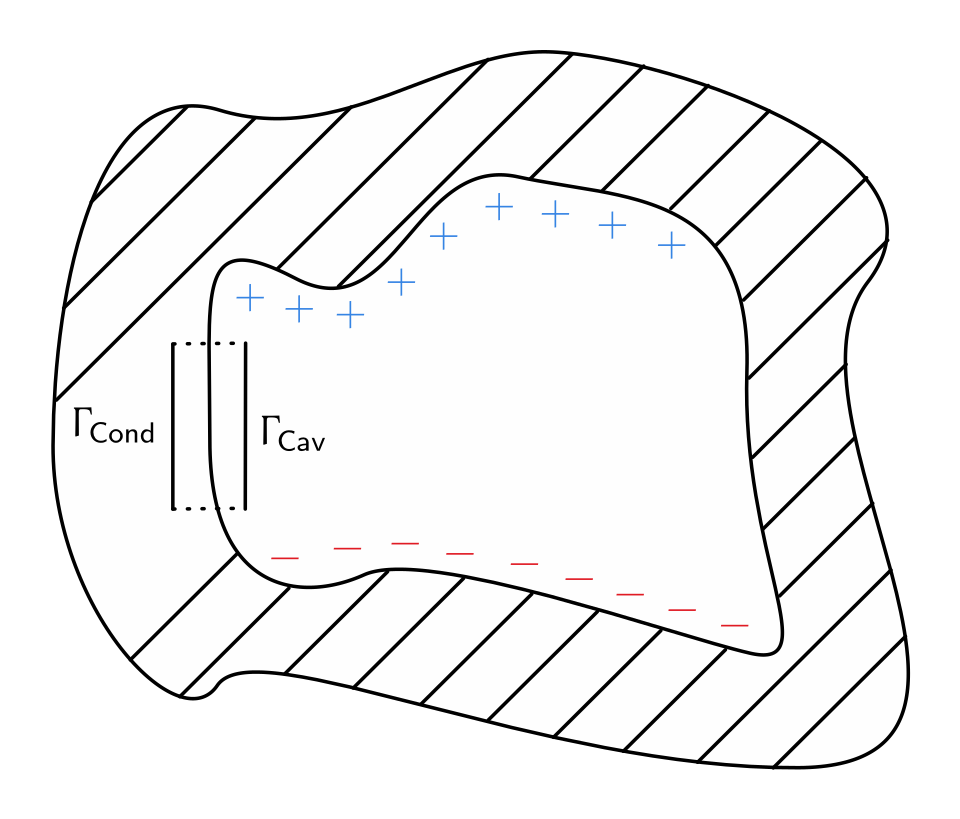
\includegraphics[width=0.6\textwidth]{dim_conduttore_cavita}
      \caption{Dimostrazione del campo nullo in un conduttore con cavità}
    \end{figure}
    per l'equazione di Maxwell sapppiamo che:
    \[
      \int_\Gamma E \cdot dl = \int_{\Gamma_{\text{Conduttore}}} E +
      \underbrace{\cancel{\int_{\Gamma_{\text{Cavità}}} E}}_{=0} \neq 0
    \] 
    E questo è assurdo, quindi il campo è nullo.
\end{enumerate}
Le linee di campo sono:
\begin{figure}[H]
  \centering
  \includegraphics[width=0.6\textwidth]{linee_campo_conduttore_cavita}
  \caption{Linee di campo in un conduttore con cavità}
\end{figure}
\noindent
Questa superficie con una cavità agisce come uno \textbf{schermo elettrostatico} (
o gabbia di Faraday) perchè il campo all'interno è nullo. 

\vspace{1em}
\noindent
Consideriamo ora un conduttore con una cavità \textbf{carica}, ciò vuol dire che
nella cavità è presente un conduttore carico e questa carica si distribuisce sulla
superficie:
\begin{figure}[H]
  \centering
  \includegraphics[width=0.6\textwidth]{conduttore_cavita_carica}
  \caption{Conduttore con una cavità carica}
\end{figure}
\noindent
Per Gauss posiziono una superficie all'interno del conduttore con la cavità, quindi:
\begin{figure}[H]
  \centering
  \includegraphics[width=0.6\textwidth]{superficie_gauss_conduttore_cavita_carica}
  \caption{Superficie di Gauss in un conduttore con cavità carica}
\end{figure}
\[
  \oint_S \underbrace{\vec{E}}_{=0} \cdot d\vec{S} = 0 = \frac{Q_{\text{int}}}{\varepsilon_0}
\] 
Visto che la carica deve essere 0, compare \textbf{per induzione} una carica uguale
ed opposta a quella della cavità:
\[
  Q_{\text{Indotta}} = - Q_{\text{Cavità}}
\]
Però la carica si conserva, quindi compare sempre per induzione una carica \( Q \)
sulla superficie esterna:
\begin{figure}[H]
  \centering
  \includegraphics[width=0.6\textwidth]{induzione_conduttore_cavita_carica}
  \caption{Induzione in un conduttore con cavità carica}
\end{figure}
\noindent
Le linee di campo sono:
\begin{figure}[H]
  \centering
  \includegraphics[width=0.6\textwidth]{linee_campo_conduttore_cavita_carica}
  \caption{Linee di campo in un conduttore con cavità carica}
\end{figure}
\noindent
Se viene aggiunta una carica all'esterno il sistema \textbf{nella cavità} non cambia
perchè la superficie agisce come uno schermo. All'esterno invece le cariche si sommano.

\begin{example}
  Consideriamo il seguente sistema:
  \begin{figure}[H]
    \centering
    \includegraphics[width=0.5\textwidth]{conduttore_cavita_sferica_carica}
    \caption{Conduttore con cavità sferica carica}
  \end{figure}
  \noindent
  Se si mette al contatto il conduttore interno con il conduttore esterno si ottiene il
  sistema del conduttore con una cavità perchè i due conduttori agiscono come se fossero
  uno solo:
  \begin{figure}[H]
    \centering
    \includegraphics[width=0.5\textwidth]{conduttore_cavita_sferica_carica_2}
    \caption{Trasformazione del condensatore in un conduttore con cavità carica}
  \end{figure}
\end{example}

\subsection{Capacità elettrostatica}
Un carica \( \{dq\}  \) genera un campo
\[
  d\vec{E} = \frac{\{dq\}}{4 \pi \varepsilon _0} \frac{\hat{r}}{r^2} \quad \left[ \frac{V}{m} \right]
\]
e un potenziale
\[
  dV = \frac{\{dq\}}{4 \pi \varepsilon_0 r} \quad \left[ V \right]
\] 
Osserviamo che c'è una linearità tra la carica e il potenziale, quindi \( V \) è
proporzionale a \( Q \) e il coefficiente di proporzionalità è la \textbf{capacità}.

\subsubsection{Conduttore isolato}
Consideriamo un qualsiasi conduttore isolato con una carica \( Q \) e un potenziale
\( V \) costante.

\begin{definition}
  Si definisce \textbf{capacità elettrostatica} \( C \) di un conduttore isolato la
  quantità di carica \( Q \) tarsferita al conduttore da un potenziale \( V \)
  \[
    C = \frac{Q}{V} \quad \left[ F \right] \text{ (Farad)}
  \]
  La capacità dipende solo dalla geometria e dal materiale.
\end{definition}

\subsubsection{Conduttore non isolato}
Consideriamo due conduttori, uno con carica \( Q \) e uno con carica \( -Q \) in
\textbf{induzione completa}, cioè tutte le linee di campo del primo oggetto vanno nel
secondo oggetto. Per avere ciò bisogna eliminare ogni interazione con l'esterno e l'unica
opzione è inserire il primo oggetto nella cavità del secondo.
\begin{figure}[H]
  \centering
  \includegraphics[width=0.5\textwidth]{conduttore_isolato}
  \caption{Isolamento di un conduttore}
\end{figure}
\noindent
Un \textbf{Condensatore} è un sistema di due conduttori in induzione completa. In
un condensatore i due conduttori si dicono \textbf{armature} o \textbf{lastre}.

\vspace{1em}
\noindent
Nella pratica si distinguono 3 casi (in questo corso):
\begin{enumerate}
  \item \textbf{Condensatore sferico}: Si hanno due sfere, una nella concavità 
    dell'altra
    \begin{figure}[H]
      \centering
      \includegraphics[width=0.5\textwidth]{condensatore_sferico}
      \caption{Condensatore sferico}
    \end{figure}

  \item \textbf{Condensatore cilindrico}: È una struttura tubolare, in cui
    se il raggio è molto minore della lunghezza del tubo allora si può \textbf{approssimare}
    come un induzione completa:
    \begin{figure}[H]
      \centering
      \includegraphics[width=0.5\textwidth]{condensatore_cilindrico}
      \caption{Condensatore cilindrico}
    \end{figure}

  \item \textbf{Condensatore piano}: È formato da due lastre piane parallele
    separate da una distanza \( h \) con una certa area \( A \). Anche in questo
    caso se le lastre sono molto grandi rispetto alla distanza si può approssimare
    come un induzione completa.
    \begin{figure}[H]
      \centering
      \includegraphics[width=0.7\textwidth]{condensatore_piano}
      \caption{Condensatore piano}
    \end{figure}
\end{enumerate}

\subsubsection{Capacità nei condensatori}
Consideriamo un condensatore:
\begin{figure}[H]
  \centering
  \includegraphics[width=0.5\textwidth]{potenziale_condensatore_sferico}
  \caption{Condensatore sferico}
\end{figure}
\noindent
La capacità è:
\[
  C = \frac{Q}{\Delta V} \quad \text{(presa positiva)}
\] 

\begin{example}
  Calcoliamo la capacità del condensatore piano nel vuoto, indicato con il seguente simbolo:
  \begin{figure}[H]
    \centering
    \begin{circuitikz}
      \draw (0,0) to[C] (2,0);
    \end{circuitikz}
    \caption{Condensatore piano}
  \end{figure}
  \noindent
  Consideriamo un piano con carica positiva e uno con carica negativa e area \( A \):
  \begin{figure}[H]
    \centering
    \includegraphics[width=0.7\textwidth]{potenziale_condensatore_piano}
    \caption{Potenziale di un condensatore piano}
  \end{figure}
  \noindent
  Il campo è solo all'interno e vale:
  \[
    E = \frac{\sigma}{\varepsilon_0}
  \] 
  La capacità è:
  \[
    C = \frac{Q}{V^+ - V^-}
  \] 
  Ora bisogna calcolare la differenza di potenziale tra le due lastre ricordando la
  definizione di potenziale:
  \[
    V_2 - V_1 = -\int_1^2 \vec{E} \cdot d\vec{l}
  \] 
  quindi
  (Il campo è negatico perchè la sua direzione è opposta a quella del potenziale):
  \[
    V^+ - V^- = - \int_-^+ \left( - \frac{\sigma}{\varepsilon_0} \right) dx 
    = \frac{\sigma }{\varepsilon _0} h \quad \left[ V \right]
  \] 
  Di conseguenza la capacità è:
  \[
    C = \frac{Q}{\frac{\sigma}{\varepsilon_0} h} = \frac{\sigma A}{\frac{\sigma}{\varepsilon_0} h}
    = \frac{\varepsilon_0 A}{h} \quad \left[ F \right]
  \]
\end{example}

\subsection{Calcolo del campo potenziale}
\subsubsection{Simmetria sferica}
Il campo di una superficie sferica è:
\[
  \vec{E} =
  \begin{cases}
    \frac{Q}{4 \pi \varepsilon_0 r^2} \hat{r} & r \ge R\\
    0 & r < R
  \end{cases}
\] 
La definizione di potenziale è:
\[
  V(r) - V_{\text{Riferimento}} = - \int_{\gamma }\vec{E} \cdot d\vec{l}
  = -\int_{\vec{r_0}}^{\vec{r}} \vec{E}(r) \, dr
\] 
dove \( V_{\text{Riferimento}} = V(rif) \to V(\infty) = 0 \). Il potenziale di reiferimento
\textbf{può} essere preso all'infinito soltanto per sistemi in cui \textbf{non} ci sono
cariche all'infinito.

Quindi il calcolo del potenziale diventa:
\[
  V(r) - \underset{=0}{\cancel{V_{\text{Riferimento}}}}
  = - \int_{\infty}^{r} \frac{Q}{4 \pi \varepsilon_0 r^2} \, dr
  = - \left.\left( \frac{-Q}{4 \pi \varepsilon_0 r} \right)\right|_{\infty}^{r}
    = \frac{Q}{4 \pi \varepsilon_0 r} \quad \left[ V \right]
\] 
(solo per \( r > R \)). Il grafico è:
\begin{figure}[H]
  \centering
  \includegraphics[width=0.9\textwidth]{grafico_potenziale}
  \caption{Grafico del potenziale}
\end{figure}

\begin{definition}
  Il potenziale si calcola come:
  \[
    V(r) =
    \begin{cases}
      \frac{Q}{4 \pi \varepsilon_0 r} & r \ge R\\
      \text{Costante} & r < R
    \end{cases}
  \] 
\end{definition}

\vspace{1em}
\noindent
Con il potenziale si può calcolare la capacita come:
\[
  C = \frac{Q}{V_{\text{Sup}}} = \frac{Q}{\frac{Q}{4 \pi \varepsilon_0 R}}
  = 4 \pi \varepsilon_0 R \quad \left[ F \right]
\] 

\begin{example}[Potenziale di un condensatore sferico]
  Consideriamo un condensatore sferico con carica \( Q \) in cui il raggio del conduttore
  sferico interno è \( R_1 \) e i raggi del conduttore sferico sono \( R_2 \) e \( R_3 \).
  Il campo è:
  \[
    \vec{E} = \frac{Q}{4 \pi \varepsilon_0 r^2} \hat{r} \quad R_1 < r < R_2
  \] 
  Il campo è nullo nei seguenti casi:
  \[
    \vec{E} = 0 \to \begin{cases}
      r < R_1\\
      R_2 < r < R_3
    \end{cases}
  \] 
  quindi all'interno del conduttore.

  Il potenziale sarà:
  \[
    V(r) = \frac{Q}{4 \pi \varepsilon_0 r} \quad \left[ V \right] \quad \text{Nella cavità}
  \] 
  All'interno dei conduttori il potenziale vale:
  \[
    \begin{aligned}
      V(R_1) &= \frac{Q}{4 \pi \varepsilon_0 R_1}\\
      V(R_2) &= \frac{Q}{4 \pi \varepsilon_0 R_2}
    \end{aligned}
  \] 
  La capacità è:
  \[
    C = \frac{Q}{\Delta V} = \frac{Q}{V(R_2) - V(R_1)}
    = \frac{Q}{\frac{Q}{4 \pi \varepsilon_0 \left( \frac{1}{R_1} - \frac{1}{R_2} \right)}}
    = 4 \pi \varepsilon_0 \frac{R_1 R_2}{R_2 - R_1} \quad \left[ F \right]
  \] 
\end{example}
\begin{example}[Potenziale in un filo indefinito]
  Consideriamo un filo indefinito conduttore con carica \( \lambda \). Il campo
  è:
  \[
    \vec{E} = \frac{\lambda}{2 \pi \varepsilon_0 r}
  \] 
  Il potenziale è calcolato come:
  \[
    V(r) - \underset{=0}{\cancel{V(rif)}} = - \int_{rif}^r \frac{\lambda}{2 \pi \varepsilon_0 r} \, dr
    = - \frac{\lambda}{2 \pi \varepsilon_0} \left( \ln(r) - \ln(rif) \right) 
  \] 
  Vogliamo che il punto di riferimento renda nullo il potenziale, quindi:
  \[
    V(rif) = 0
  \] 
  quindi il punto di riferimento è un punto qualunque
  \[
    rif \neq \infty
  \] 
  Il grafico del potenziale è:
  \begin{figure}[H]
    \centering
    \includegraphics[width=0.9\textwidth]{grafico_potenziale_filo}
    \caption{Grafico del potenziale}
  \end{figure}
\end{example}

\end{document}
